\documentclass[twoside]{book}

% Packages required by doxygen
\usepackage{fixltx2e}
\usepackage{calc}
\usepackage{doxygen}
\usepackage[export]{adjustbox} % also loads graphicx
\usepackage{graphicx}
\usepackage[utf8]{inputenc}
\usepackage{makeidx}
\usepackage{multicol}
\usepackage{multirow}
\PassOptionsToPackage{warn}{textcomp}
\usepackage{textcomp}
\usepackage[nointegrals]{wasysym}
\usepackage[table]{xcolor}

% Font selection
\usepackage[T1]{fontenc}
\usepackage[scaled=.90]{helvet}
\usepackage{courier}
\usepackage{amssymb}
\usepackage{sectsty}
\renewcommand{\familydefault}{\sfdefault}
\allsectionsfont{%
  \fontseries{bc}\selectfont%
  \color{darkgray}%
}
\renewcommand{\DoxyLabelFont}{%
  \fontseries{bc}\selectfont%
  \color{darkgray}%
}
\newcommand{\+}{\discretionary{\mbox{\scriptsize$\hookleftarrow$}}{}{}}

% Page & text layout
\usepackage{geometry}
\geometry{%
  a4paper,%
  top=2.5cm,%
  bottom=2.5cm,%
  left=2.5cm,%
  right=2.5cm%
}
\tolerance=750
\hfuzz=15pt
\hbadness=750
\setlength{\emergencystretch}{15pt}
\setlength{\parindent}{0cm}
\setlength{\parskip}{3ex plus 2ex minus 2ex}
\makeatletter
\renewcommand{\paragraph}{%
  \@startsection{paragraph}{4}{0ex}{-1.0ex}{1.0ex}{%
    \normalfont\normalsize\bfseries\SS@parafont%
  }%
}
\renewcommand{\subparagraph}{%
  \@startsection{subparagraph}{5}{0ex}{-1.0ex}{1.0ex}{%
    \normalfont\normalsize\bfseries\SS@subparafont%
  }%
}
\makeatother

% Headers & footers
\usepackage{fancyhdr}
\pagestyle{fancyplain}
\fancyhead[LE]{\fancyplain{}{\bfseries\thepage}}
\fancyhead[CE]{\fancyplain{}{}}
\fancyhead[RE]{\fancyplain{}{\bfseries\leftmark}}
\fancyhead[LO]{\fancyplain{}{\bfseries\rightmark}}
\fancyhead[CO]{\fancyplain{}{}}
\fancyhead[RO]{\fancyplain{}{\bfseries\thepage}}
\fancyfoot[LE]{\fancyplain{}{}}
\fancyfoot[CE]{\fancyplain{}{}}
\fancyfoot[RE]{\fancyplain{}{\bfseries\scriptsize Generated by Doxygen }}
\fancyfoot[LO]{\fancyplain{}{\bfseries\scriptsize Generated by Doxygen }}
\fancyfoot[CO]{\fancyplain{}{}}
\fancyfoot[RO]{\fancyplain{}{}}
\renewcommand{\footrulewidth}{0.4pt}
\renewcommand{\chaptermark}[1]{%
  \markboth{#1}{}%
}
\renewcommand{\sectionmark}[1]{%
  \markright{\thesection\ #1}%
}

% Indices & bibliography
\usepackage{natbib}
\usepackage[titles]{tocloft}
\setcounter{tocdepth}{3}
\setcounter{secnumdepth}{5}
\makeindex

% Hyperlinks (required, but should be loaded last)
\usepackage{ifpdf}
\ifpdf
  \usepackage[pdftex,pagebackref=true]{hyperref}
\else
  \usepackage[ps2pdf,pagebackref=true]{hyperref}
\fi
\hypersetup{%
  colorlinks=true,%
  linkcolor=blue,%
  citecolor=blue,%
  unicode%
}

% Custom commands
\newcommand{\clearemptydoublepage}{%
  \newpage{\pagestyle{empty}\cleardoublepage}%
}

\usepackage{caption}
\captionsetup{labelsep=space,justification=centering,font={bf},singlelinecheck=off,skip=4pt,position=top}

%===== C O N T E N T S =====

\begin{document}

% Titlepage & ToC
\hypersetup{pageanchor=false,
             bookmarksnumbered=true,
             pdfencoding=unicode
            }
\pagenumbering{alph}
\begin{titlepage}
\vspace*{7cm}
\begin{center}%
{\Large A place in the Sun \\[1ex]\large 1.\+0 }\\
\vspace*{1cm}
{\large Generated by Doxygen 1.8.12}\\
\end{center}
\end{titlepage}
\clearemptydoublepage
\pagenumbering{roman}
\tableofcontents
\clearemptydoublepage
\pagenumbering{arabic}
\hypersetup{pageanchor=true}

%--- Begin generated contents ---
\chapter{Hierarchical Index}
\section{Class Hierarchy}
This inheritance list is sorted roughly, but not completely, alphabetically\+:\begin{DoxyCompactList}
\item \contentsline{section}{Accomodation}{\pageref{class_accomodation}}{}
\begin{DoxyCompactList}
\item \contentsline{section}{Apartment}{\pageref{class_apartment}}{}
\item \contentsline{section}{Bedroom}{\pageref{class_bedroom}}{}
\item \contentsline{section}{Flat}{\pageref{class_flat}}{}
\end{DoxyCompactList}
\item \contentsline{section}{Company}{\pageref{class_company}}{}
\item \contentsline{section}{Date}{\pageref{class_date}}{}
\item \contentsline{section}{Error\+Opening\+File}{\pageref{class_error_opening_file}}{}
\item \contentsline{section}{Invalid\+Date}{\pageref{class_invalid_date}}{}
\item \contentsline{section}{Invalid\+Input}{\pageref{class_invalid_input}}{}
\item \contentsline{section}{Invalid\+Log\+In}{\pageref{class_invalid_log_in}}{}
\item \contentsline{section}{Invalid\+Reservation\+ID}{\pageref{class_invalid_reservation_i_d}}{}
\item \contentsline{section}{Invalid\+Username}{\pageref{class_invalid_username}}{}
\item \contentsline{section}{Reservation}{\pageref{class_reservation}}{}
\item \contentsline{section}{User}{\pageref{class_user}}{}
\begin{DoxyCompactList}
\item \contentsline{section}{Client}{\pageref{class_client}}{}
\item \contentsline{section}{Suplier}{\pageref{class_suplier}}{}
\end{DoxyCompactList}
\item \contentsline{section}{Wrong\+Option}{\pageref{class_wrong_option}}{}
\end{DoxyCompactList}

\chapter{Class Index}
\section{Class List}
Here are the classes, structs, unions and interfaces with brief descriptions\+:\begin{DoxyCompactList}
\item\contentsline{section}{\hyperlink{class_accomodation}{Accomodation} }{\pageref{class_accomodation}}{}
\item\contentsline{section}{\hyperlink{class_apartment}{Apartment} }{\pageref{class_apartment}}{}
\item\contentsline{section}{\hyperlink{class_bedroom}{Bedroom} }{\pageref{class_bedroom}}{}
\item\contentsline{section}{\hyperlink{class_client}{Client} }{\pageref{class_client}}{}
\item\contentsline{section}{\hyperlink{class_company}{Company} }{\pageref{class_company}}{}
\item\contentsline{section}{\hyperlink{class_date}{Date} }{\pageref{class_date}}{}
\item\contentsline{section}{\hyperlink{class_error_opening_file}{Error\+Opening\+File} }{\pageref{class_error_opening_file}}{}
\item\contentsline{section}{\hyperlink{class_flat}{Flat} }{\pageref{class_flat}}{}
\item\contentsline{section}{\hyperlink{class_invalid_date}{Invalid\+Date} }{\pageref{class_invalid_date}}{}
\item\contentsline{section}{\hyperlink{class_invalid_input}{Invalid\+Input} }{\pageref{class_invalid_input}}{}
\item\contentsline{section}{\hyperlink{class_invalid_log_in}{Invalid\+Log\+In} }{\pageref{class_invalid_log_in}}{}
\item\contentsline{section}{\hyperlink{class_invalid_reservation_i_d}{Invalid\+Reservation\+ID} }{\pageref{class_invalid_reservation_i_d}}{}
\item\contentsline{section}{\hyperlink{class_invalid_username}{Invalid\+Username} }{\pageref{class_invalid_username}}{}
\item\contentsline{section}{\hyperlink{class_reservation}{Reservation} }{\pageref{class_reservation}}{}
\item\contentsline{section}{\hyperlink{class_suplier}{Suplier} }{\pageref{class_suplier}}{}
\item\contentsline{section}{\hyperlink{class_user}{User} }{\pageref{class_user}}{}
\item\contentsline{section}{\hyperlink{class_wrong_option}{Wrong\+Option} }{\pageref{class_wrong_option}}{}
\end{DoxyCompactList}

\chapter{Class Documentation}
\hypertarget{class_accomodation}{}\section{Accomodation Class Reference}
\label{class_accomodation}\index{Accomodation@{Accomodation}}
Inheritance diagram for Accomodation\+:\begin{figure}[H]
\begin{center}
\leavevmode
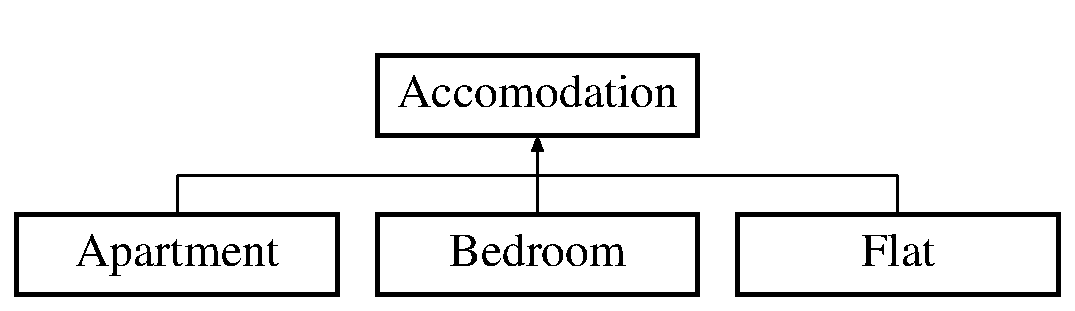
\includegraphics[height=2.000000cm]{class_accomodation}
\end{center}
\end{figure}
\subsection*{Public Member Functions}
\begin{DoxyCompactItemize}
\item 
\hyperlink{class_accomodation_a6f9d474e6bf2cd77d0046c3584a50bc6}{Accomodation} (float price\+\_\+night, float price\+\_\+week, float price\+\_\+month, string location, vector$<$ pair$<$ \hyperlink{class_date}{Date}, \hyperlink{class_date}{Date} $>$$>$ available\+\_\+dates)
\begin{DoxyCompactList}\small\item\em accomodation constructor \end{DoxyCompactList}\item 
\hyperlink{class_accomodation_a1e9a337679884eeb358e998a26c7e98b}{Accomodation} (unsigned int id, float price\+\_\+night, float price\+\_\+week, float price\+\_\+month, string location, vector$<$ pair$<$ \hyperlink{class_date}{Date}, \hyperlink{class_date}{Date} $>$$>$ available\+\_\+dates)
\begin{DoxyCompactList}\small\item\em accomodation constructor with id \end{DoxyCompactList}\item 
float \hyperlink{class_accomodation_a9061a7cadf76377cbab25043e53ef5ef}{get\+Price\+Night} () const
\begin{DoxyCompactList}\small\item\em gets price\+\_\+night \end{DoxyCompactList}\item 
float \hyperlink{class_accomodation_ab466bd7dc51b8f48ac4e9152c96c95f7}{get\+Price\+Week} () const
\begin{DoxyCompactList}\small\item\em gets price\+\_\+week \end{DoxyCompactList}\item 
float \hyperlink{class_accomodation_a3e58fd8b7a752fb7c8709fcb979cfbb5}{get\+Price\+Month} () const
\begin{DoxyCompactList}\small\item\em gets price\+\_\+month \end{DoxyCompactList}\item 
string \hyperlink{class_accomodation_a4412dad54b791d4db1ebd01176c1333e}{get\+Location} () const
\begin{DoxyCompactList}\small\item\em gets location \end{DoxyCompactList}\item 
unsigned int \hyperlink{class_accomodation_a04d05660220ad6ad31619bdf9bab28e9}{get\+ID} () const
\begin{DoxyCompactList}\small\item\em gets ID \end{DoxyCompactList}\item 
void \hyperlink{class_accomodation_a3d06b872d484b5aa2455d65d98b63645}{set\+ID} (unsigned int id)
\begin{DoxyCompactList}\small\item\em sets ID \end{DoxyCompactList}\item 
virtual void \hyperlink{class_accomodation_a4394eb907b2d5a23faf73dd03c1dac4d}{save\+Accomodation} (ofstream \&out)
\begin{DoxyCompactList}\small\item\em virtual fuction to save accomodation on the supliers file \end{DoxyCompactList}\item 
float \hyperlink{class_accomodation_aa37ad0d3356128f880c00b647d2f2bff}{get\+Fee} ()
\begin{DoxyCompactList}\small\item\em gets fee \end{DoxyCompactList}\item 
void \hyperlink{class_accomodation_a9fc9164c6a0a353538e422ec36db43f4}{set\+Fee} (float fee)
\begin{DoxyCompactList}\small\item\em sets fee \end{DoxyCompactList}\item 
void \hyperlink{class_accomodation_aefbbf86e80b202ca4879fb695cdb7d3d}{add\+Dates} (const pair$<$ \hyperlink{class_date}{Date}, \hyperlink{class_date}{Date} $>$ \&dates)
\begin{DoxyCompactList}\small\item\em adds dates to the vector of unavailable dates \end{DoxyCompactList}\item 
void \hyperlink{class_accomodation_ad77bdf46460657e8670001c91bce72b3}{remove\+Dates} (\hyperlink{class_date}{Date} check\+IN, \hyperlink{class_date}{Date} check\+O\+UT)
\begin{DoxyCompactList}\small\item\em removes dates to the vector of unavailable dates \end{DoxyCompactList}\item 
vector$<$ pair$<$ \hyperlink{class_date}{Date}, \hyperlink{class_date}{Date} $>$ $>$ \hyperlink{class_accomodation_a63c58fd6e01101095522573579490e7b}{get\+Unavailable\+Dates} () const
\begin{DoxyCompactList}\small\item\em gets unavailable dates \end{DoxyCompactList}\item 
\hypertarget{class_accomodation_ac38668edd6b7cd608dc9e8ab9a780efb}{}\label{class_accomodation_ac38668edd6b7cd608dc9e8ab9a780efb} 
virtual void \hyperlink{class_accomodation_ac38668edd6b7cd608dc9e8ab9a780efb}{print} () const
\begin{DoxyCompactList}\small\item\em virtual fuction to print a accomodation on the screen \end{DoxyCompactList}\item 
bool \hyperlink{class_accomodation_ae42299afc3f8bf211fe69821f876d48a}{operator==} (const \hyperlink{class_accomodation}{Accomodation} \&acc) const
\begin{DoxyCompactList}\small\item\em overload of the the equality operator \end{DoxyCompactList}\end{DoxyCompactItemize}
\subsection*{Static Public Member Functions}
\begin{DoxyCompactItemize}
\item 
static unsigned int \hyperlink{class_accomodation_a2ceca7929ed995f3fdc40e3d6b7e017c}{get\+Last\+ID} ()
\begin{DoxyCompactList}\small\item\em gets last\+ID \end{DoxyCompactList}\item 
static void \hyperlink{class_accomodation_a5554cdc8b46ae1fb92c94bf4696f9b77}{set\+Acc\+Last\+ID} (unsigned int id)
\begin{DoxyCompactList}\small\item\em sets accomomodation last id \end{DoxyCompactList}\end{DoxyCompactItemize}


\subsection{Constructor \& Destructor Documentation}
\hypertarget{class_accomodation_a6f9d474e6bf2cd77d0046c3584a50bc6}{}\label{class_accomodation_a6f9d474e6bf2cd77d0046c3584a50bc6} 
\index{Accomodation@{Accomodation}!Accomodation@{Accomodation}}
\index{Accomodation@{Accomodation}!Accomodation@{Accomodation}}
\subsubsection{\texorpdfstring{Accomodation()}{Accomodation()}\hspace{0.1cm}{\footnotesize\ttfamily [1/2]}}
{\footnotesize\ttfamily Accomodation\+::\+Accomodation (\begin{DoxyParamCaption}\item[{float}]{price\+\_\+night,  }\item[{float}]{price\+\_\+week,  }\item[{float}]{price\+\_\+month,  }\item[{string}]{location,  }\item[{vector$<$ pair$<$ \hyperlink{class_date}{Date}, \hyperlink{class_date}{Date} $>$$>$}]{available\+\_\+dates }\end{DoxyParamCaption})}



accomodation constructor 


\begin{DoxyParams}{Parameters}
{\em price\+\_\+night} & \\
\hline
{\em price\+\_\+week} & \\
\hline
{\em price\+\_\+month} & \\
\hline
{\em location} & \\
\hline
{\em unavailable\+\_\+dates} & \\
\hline
\end{DoxyParams}
\hypertarget{class_accomodation_a1e9a337679884eeb358e998a26c7e98b}{}\label{class_accomodation_a1e9a337679884eeb358e998a26c7e98b} 
\index{Accomodation@{Accomodation}!Accomodation@{Accomodation}}
\index{Accomodation@{Accomodation}!Accomodation@{Accomodation}}
\subsubsection{\texorpdfstring{Accomodation()}{Accomodation()}\hspace{0.1cm}{\footnotesize\ttfamily [2/2]}}
{\footnotesize\ttfamily Accomodation\+::\+Accomodation (\begin{DoxyParamCaption}\item[{unsigned int}]{id,  }\item[{float}]{price\+\_\+night,  }\item[{float}]{price\+\_\+week,  }\item[{float}]{price\+\_\+month,  }\item[{string}]{location,  }\item[{vector$<$ pair$<$ \hyperlink{class_date}{Date}, \hyperlink{class_date}{Date} $>$$>$}]{available\+\_\+dates }\end{DoxyParamCaption})}



accomodation constructor with id 


\begin{DoxyParams}{Parameters}
{\em id} & \\
\hline
{\em price\+\_\+night} & \\
\hline
{\em price\+\_\+week} & \\
\hline
{\em price\+\_\+month} & \\
\hline
{\em location} & \\
\hline
{\em unavailable\+\_\+dates} & \\
\hline
\end{DoxyParams}


\subsection{Member Function Documentation}
\hypertarget{class_accomodation_aefbbf86e80b202ca4879fb695cdb7d3d}{}\label{class_accomodation_aefbbf86e80b202ca4879fb695cdb7d3d} 
\index{Accomodation@{Accomodation}!add\+Dates@{add\+Dates}}
\index{add\+Dates@{add\+Dates}!Accomodation@{Accomodation}}
\subsubsection{\texorpdfstring{add\+Dates()}{addDates()}}
{\footnotesize\ttfamily void Accomodation\+::add\+Dates (\begin{DoxyParamCaption}\item[{const pair$<$ \hyperlink{class_date}{Date}, \hyperlink{class_date}{Date} $>$ \&}]{dates }\end{DoxyParamCaption})}



adds dates to the vector of unavailable dates 


\begin{DoxyParams}{Parameters}
{\em dates} & pair of dates(initial and final) \\
\hline
\end{DoxyParams}
\hypertarget{class_accomodation_aa37ad0d3356128f880c00b647d2f2bff}{}\label{class_accomodation_aa37ad0d3356128f880c00b647d2f2bff} 
\index{Accomodation@{Accomodation}!get\+Fee@{get\+Fee}}
\index{get\+Fee@{get\+Fee}!Accomodation@{Accomodation}}
\subsubsection{\texorpdfstring{get\+Fee()}{getFee()}}
{\footnotesize\ttfamily float Accomodation\+::get\+Fee (\begin{DoxyParamCaption}{ }\end{DoxyParamCaption})\hspace{0.3cm}{\ttfamily [inline]}}



gets fee 

\begin{DoxyReturn}{Returns}
fee that supliers pay for each reservations 
\end{DoxyReturn}
\hypertarget{class_accomodation_a04d05660220ad6ad31619bdf9bab28e9}{}\label{class_accomodation_a04d05660220ad6ad31619bdf9bab28e9} 
\index{Accomodation@{Accomodation}!get\+ID@{get\+ID}}
\index{get\+ID@{get\+ID}!Accomodation@{Accomodation}}
\subsubsection{\texorpdfstring{get\+I\+D()}{getID()}}
{\footnotesize\ttfamily unsigned int Accomodation\+::get\+ID (\begin{DoxyParamCaption}{ }\end{DoxyParamCaption}) const\hspace{0.3cm}{\ttfamily [inline]}}



gets ID 

\begin{DoxyReturn}{Returns}
ID 
\end{DoxyReturn}
\hypertarget{class_accomodation_a2ceca7929ed995f3fdc40e3d6b7e017c}{}\label{class_accomodation_a2ceca7929ed995f3fdc40e3d6b7e017c} 
\index{Accomodation@{Accomodation}!get\+Last\+ID@{get\+Last\+ID}}
\index{get\+Last\+ID@{get\+Last\+ID}!Accomodation@{Accomodation}}
\subsubsection{\texorpdfstring{get\+Last\+I\+D()}{getLastID()}}
{\footnotesize\ttfamily static unsigned int Accomodation\+::get\+Last\+ID (\begin{DoxyParamCaption}{ }\end{DoxyParamCaption})\hspace{0.3cm}{\ttfamily [inline]}, {\ttfamily [static]}}



gets last\+ID 

\begin{DoxyReturn}{Returns}
last\+ID 
\end{DoxyReturn}
\hypertarget{class_accomodation_a4412dad54b791d4db1ebd01176c1333e}{}\label{class_accomodation_a4412dad54b791d4db1ebd01176c1333e} 
\index{Accomodation@{Accomodation}!get\+Location@{get\+Location}}
\index{get\+Location@{get\+Location}!Accomodation@{Accomodation}}
\subsubsection{\texorpdfstring{get\+Location()}{getLocation()}}
{\footnotesize\ttfamily string Accomodation\+::get\+Location (\begin{DoxyParamCaption}{ }\end{DoxyParamCaption}) const\hspace{0.3cm}{\ttfamily [inline]}}



gets location 

\begin{DoxyReturn}{Returns}
location 
\end{DoxyReturn}
\hypertarget{class_accomodation_a3e58fd8b7a752fb7c8709fcb979cfbb5}{}\label{class_accomodation_a3e58fd8b7a752fb7c8709fcb979cfbb5} 
\index{Accomodation@{Accomodation}!get\+Price\+Month@{get\+Price\+Month}}
\index{get\+Price\+Month@{get\+Price\+Month}!Accomodation@{Accomodation}}
\subsubsection{\texorpdfstring{get\+Price\+Month()}{getPriceMonth()}}
{\footnotesize\ttfamily float Accomodation\+::get\+Price\+Month (\begin{DoxyParamCaption}{ }\end{DoxyParamCaption}) const\hspace{0.3cm}{\ttfamily [inline]}}



gets price\+\_\+month 

\begin{DoxyReturn}{Returns}
price\+\_\+month 
\end{DoxyReturn}
\hypertarget{class_accomodation_a9061a7cadf76377cbab25043e53ef5ef}{}\label{class_accomodation_a9061a7cadf76377cbab25043e53ef5ef} 
\index{Accomodation@{Accomodation}!get\+Price\+Night@{get\+Price\+Night}}
\index{get\+Price\+Night@{get\+Price\+Night}!Accomodation@{Accomodation}}
\subsubsection{\texorpdfstring{get\+Price\+Night()}{getPriceNight()}}
{\footnotesize\ttfamily float Accomodation\+::get\+Price\+Night (\begin{DoxyParamCaption}{ }\end{DoxyParamCaption}) const\hspace{0.3cm}{\ttfamily [inline]}}



gets price\+\_\+night 

\begin{DoxyReturn}{Returns}
price\+\_\+night 
\end{DoxyReturn}
\hypertarget{class_accomodation_ab466bd7dc51b8f48ac4e9152c96c95f7}{}\label{class_accomodation_ab466bd7dc51b8f48ac4e9152c96c95f7} 
\index{Accomodation@{Accomodation}!get\+Price\+Week@{get\+Price\+Week}}
\index{get\+Price\+Week@{get\+Price\+Week}!Accomodation@{Accomodation}}
\subsubsection{\texorpdfstring{get\+Price\+Week()}{getPriceWeek()}}
{\footnotesize\ttfamily float Accomodation\+::get\+Price\+Week (\begin{DoxyParamCaption}{ }\end{DoxyParamCaption}) const\hspace{0.3cm}{\ttfamily [inline]}}



gets price\+\_\+week 

\begin{DoxyReturn}{Returns}
price\+\_\+week 
\end{DoxyReturn}
\hypertarget{class_accomodation_a63c58fd6e01101095522573579490e7b}{}\label{class_accomodation_a63c58fd6e01101095522573579490e7b} 
\index{Accomodation@{Accomodation}!get\+Unavailable\+Dates@{get\+Unavailable\+Dates}}
\index{get\+Unavailable\+Dates@{get\+Unavailable\+Dates}!Accomodation@{Accomodation}}
\subsubsection{\texorpdfstring{get\+Unavailable\+Dates()}{getUnavailableDates()}}
{\footnotesize\ttfamily vector$<$pair$<$\hyperlink{class_date}{Date}, \hyperlink{class_date}{Date}$>$ $>$ Accomodation\+::get\+Unavailable\+Dates (\begin{DoxyParamCaption}{ }\end{DoxyParamCaption}) const\hspace{0.3cm}{\ttfamily [inline]}}



gets unavailable dates 

\begin{DoxyReturn}{Returns}
unavailable dates 
\end{DoxyReturn}
\hypertarget{class_accomodation_ae42299afc3f8bf211fe69821f876d48a}{}\label{class_accomodation_ae42299afc3f8bf211fe69821f876d48a} 
\index{Accomodation@{Accomodation}!operator==@{operator==}}
\index{operator==@{operator==}!Accomodation@{Accomodation}}
\subsubsection{\texorpdfstring{operator==()}{operator==()}}
{\footnotesize\ttfamily bool Accomodation\+::operator== (\begin{DoxyParamCaption}\item[{const \hyperlink{class_accomodation}{Accomodation} \&}]{acc }\end{DoxyParamCaption}) const}



overload of the the equality operator 


\begin{DoxyParams}{Parameters}
{\em acc} & \\
\hline
\end{DoxyParams}
\begin{DoxyReturn}{Returns}
true is accomodations have the same id, false otherwise 
\end{DoxyReturn}
\hypertarget{class_accomodation_ad77bdf46460657e8670001c91bce72b3}{}\label{class_accomodation_ad77bdf46460657e8670001c91bce72b3} 
\index{Accomodation@{Accomodation}!remove\+Dates@{remove\+Dates}}
\index{remove\+Dates@{remove\+Dates}!Accomodation@{Accomodation}}
\subsubsection{\texorpdfstring{remove\+Dates()}{removeDates()}}
{\footnotesize\ttfamily void Accomodation\+::remove\+Dates (\begin{DoxyParamCaption}\item[{\hyperlink{class_date}{Date}}]{check\+IN,  }\item[{\hyperlink{class_date}{Date}}]{check\+O\+UT }\end{DoxyParamCaption})}



removes dates to the vector of unavailable dates 


\begin{DoxyParams}{Parameters}
{\em check\+IN} & \\
\hline
{\em check\+O\+UT} & \\
\hline
\end{DoxyParams}
\hypertarget{class_accomodation_a4394eb907b2d5a23faf73dd03c1dac4d}{}\label{class_accomodation_a4394eb907b2d5a23faf73dd03c1dac4d} 
\index{Accomodation@{Accomodation}!save\+Accomodation@{save\+Accomodation}}
\index{save\+Accomodation@{save\+Accomodation}!Accomodation@{Accomodation}}
\subsubsection{\texorpdfstring{save\+Accomodation()}{saveAccomodation()}}
{\footnotesize\ttfamily void Accomodation\+::save\+Accomodation (\begin{DoxyParamCaption}\item[{ofstream \&}]{out }\end{DoxyParamCaption})\hspace{0.3cm}{\ttfamily [virtual]}}



virtual fuction to save accomodation on the supliers file 


\begin{DoxyParams}{Parameters}
{\em out} & file supliers \\
\hline
\end{DoxyParams}


Reimplemented in \hyperlink{class_apartment_af30f7fa6ee2877315b553614dcfad9f2}{Apartment}, \hyperlink{class_flat_a9569fe297d02edebfe67d62125a86696}{Flat}, and \hyperlink{class_bedroom_ad5d0a12fe0257ba5c14efc6182ee33ce}{Bedroom}.

\hypertarget{class_accomodation_a5554cdc8b46ae1fb92c94bf4696f9b77}{}\label{class_accomodation_a5554cdc8b46ae1fb92c94bf4696f9b77} 
\index{Accomodation@{Accomodation}!set\+Acc\+Last\+ID@{set\+Acc\+Last\+ID}}
\index{set\+Acc\+Last\+ID@{set\+Acc\+Last\+ID}!Accomodation@{Accomodation}}
\subsubsection{\texorpdfstring{set\+Acc\+Last\+I\+D()}{setAccLastID()}}
{\footnotesize\ttfamily void Accomodation\+::set\+Acc\+Last\+ID (\begin{DoxyParamCaption}\item[{unsigned int}]{id }\end{DoxyParamCaption})\hspace{0.3cm}{\ttfamily [static]}}



sets accomomodation last id 


\begin{DoxyParams}{Parameters}
{\em id} & \\
\hline
\end{DoxyParams}
\hypertarget{class_accomodation_a9fc9164c6a0a353538e422ec36db43f4}{}\label{class_accomodation_a9fc9164c6a0a353538e422ec36db43f4} 
\index{Accomodation@{Accomodation}!set\+Fee@{set\+Fee}}
\index{set\+Fee@{set\+Fee}!Accomodation@{Accomodation}}
\subsubsection{\texorpdfstring{set\+Fee()}{setFee()}}
{\footnotesize\ttfamily void Accomodation\+::set\+Fee (\begin{DoxyParamCaption}\item[{float}]{fee }\end{DoxyParamCaption})\hspace{0.3cm}{\ttfamily [inline]}}



sets fee 


\begin{DoxyParams}{Parameters}
{\em fee} & \\
\hline
\end{DoxyParams}
\hypertarget{class_accomodation_a3d06b872d484b5aa2455d65d98b63645}{}\label{class_accomodation_a3d06b872d484b5aa2455d65d98b63645} 
\index{Accomodation@{Accomodation}!set\+ID@{set\+ID}}
\index{set\+ID@{set\+ID}!Accomodation@{Accomodation}}
\subsubsection{\texorpdfstring{set\+I\+D()}{setID()}}
{\footnotesize\ttfamily void Accomodation\+::set\+ID (\begin{DoxyParamCaption}\item[{unsigned int}]{id }\end{DoxyParamCaption})\hspace{0.3cm}{\ttfamily [inline]}}



sets ID 


\begin{DoxyParams}{Parameters}
{\em id} & \\
\hline
\end{DoxyParams}


The documentation for this class was generated from the following files\+:\begin{DoxyCompactItemize}
\item 
Accomodation.\+h\item 
Accomodation.\+cpp\end{DoxyCompactItemize}

\hypertarget{class_apartment}{}\section{Apartment Class Reference}
\label{class_apartment}\index{Apartment@{Apartment}}
Inheritance diagram for Apartment\+:\begin{figure}[H]
\begin{center}
\leavevmode
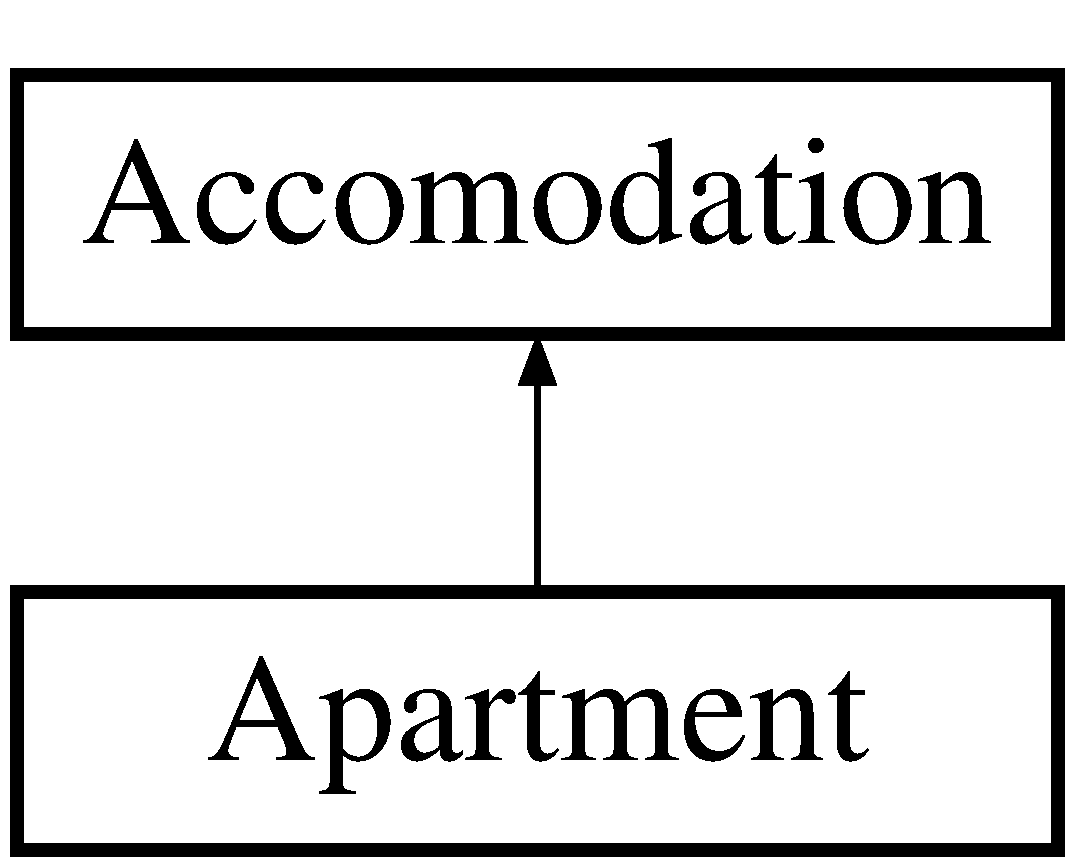
\includegraphics[height=2.000000cm]{class_apartment}
\end{center}
\end{figure}
\subsection*{Public Member Functions}
\begin{DoxyCompactItemize}
\item 
\hyperlink{class_apartment_a8851834df1a78dac09f42f67ab3feef5}{Apartment} (float price\+\_\+night, float price\+\_\+week, float price\+\_\+month, string location, vector$<$ pair$<$ \hyperlink{class_date}{Date}, \hyperlink{class_date}{Date} $>$$>$ unavailable\+\_\+dates, int n\+\_\+bed, bool suite)
\begin{DoxyCompactList}\small\item\em apartment constructor \end{DoxyCompactList}\item 
\hyperlink{class_apartment_aef273f2999734bfb67eff6bf74726db9}{Apartment} (unsigned int id, float price\+\_\+night, float price\+\_\+week, float price\+\_\+month, string location, vector$<$ pair$<$ \hyperlink{class_date}{Date}, \hyperlink{class_date}{Date} $>$$>$ unavailable\+\_\+dates, int n\+\_\+bed, bool suite)
\begin{DoxyCompactList}\small\item\em apartment constructor with id \end{DoxyCompactList}\item 
\hypertarget{class_apartment_a579261a498031a59514f3a5021a437c1}{}\label{class_apartment_a579261a498031a59514f3a5021a437c1} 
virtual void \hyperlink{class_apartment_a579261a498031a59514f3a5021a437c1}{print} () const
\begin{DoxyCompactList}\small\item\em prints apartment on the sreen \end{DoxyCompactList}\item 
virtual void \hyperlink{class_apartment_af30f7fa6ee2877315b553614dcfad9f2}{save\+Accomodation} (ofstream \&out)
\begin{DoxyCompactList}\small\item\em saves apartment in supliers file \end{DoxyCompactList}\end{DoxyCompactItemize}
\subsection*{Additional Inherited Members}


\subsection{Constructor \& Destructor Documentation}
\hypertarget{class_apartment_a8851834df1a78dac09f42f67ab3feef5}{}\label{class_apartment_a8851834df1a78dac09f42f67ab3feef5} 
\index{Apartment@{Apartment}!Apartment@{Apartment}}
\index{Apartment@{Apartment}!Apartment@{Apartment}}
\subsubsection{\texorpdfstring{Apartment()}{Apartment()}\hspace{0.1cm}{\footnotesize\ttfamily [1/2]}}
{\footnotesize\ttfamily Apartment\+::\+Apartment (\begin{DoxyParamCaption}\item[{float}]{price\+\_\+night,  }\item[{float}]{price\+\_\+week,  }\item[{float}]{price\+\_\+month,  }\item[{string}]{location,  }\item[{vector$<$ pair$<$ \hyperlink{class_date}{Date}, \hyperlink{class_date}{Date} $>$$>$}]{unavailable\+\_\+dates,  }\item[{int}]{n\+\_\+bed,  }\item[{bool}]{suite }\end{DoxyParamCaption})}



apartment constructor 


\begin{DoxyParams}{Parameters}
{\em price\+\_\+night} & \\
\hline
{\em price\+\_\+week} & \\
\hline
{\em price\+\_\+month} & \\
\hline
{\em location} & \\
\hline
{\em unavailable\+\_\+dates} & \\
\hline
\end{DoxyParams}
\hypertarget{class_apartment_aef273f2999734bfb67eff6bf74726db9}{}\label{class_apartment_aef273f2999734bfb67eff6bf74726db9} 
\index{Apartment@{Apartment}!Apartment@{Apartment}}
\index{Apartment@{Apartment}!Apartment@{Apartment}}
\subsubsection{\texorpdfstring{Apartment()}{Apartment()}\hspace{0.1cm}{\footnotesize\ttfamily [2/2]}}
{\footnotesize\ttfamily Apartment\+::\+Apartment (\begin{DoxyParamCaption}\item[{unsigned int}]{id,  }\item[{float}]{price\+\_\+night,  }\item[{float}]{price\+\_\+week,  }\item[{float}]{price\+\_\+month,  }\item[{string}]{location,  }\item[{vector$<$ pair$<$ \hyperlink{class_date}{Date}, \hyperlink{class_date}{Date} $>$$>$}]{unavailable\+\_\+dates,  }\item[{int}]{n\+\_\+bed,  }\item[{bool}]{suite }\end{DoxyParamCaption})}



apartment constructor with id 


\begin{DoxyParams}{Parameters}
{\em id} & \\
\hline
{\em price\+\_\+night} & \\
\hline
{\em price\+\_\+week} & \\
\hline
{\em price\+\_\+month} & \\
\hline
{\em location} & \\
\hline
{\em unavailable\+\_\+dates} & \\
\hline
\end{DoxyParams}


\subsection{Member Function Documentation}
\hypertarget{class_apartment_af30f7fa6ee2877315b553614dcfad9f2}{}\label{class_apartment_af30f7fa6ee2877315b553614dcfad9f2} 
\index{Apartment@{Apartment}!save\+Accomodation@{save\+Accomodation}}
\index{save\+Accomodation@{save\+Accomodation}!Apartment@{Apartment}}
\subsubsection{\texorpdfstring{save\+Accomodation()}{saveAccomodation()}}
{\footnotesize\ttfamily void Apartment\+::save\+Accomodation (\begin{DoxyParamCaption}\item[{ofstream \&}]{out }\end{DoxyParamCaption})\hspace{0.3cm}{\ttfamily [virtual]}}



saves apartment in supliers file 


\begin{DoxyParams}{Parameters}
{\em out} & supliers file \\
\hline
\end{DoxyParams}


Reimplemented from \hyperlink{class_accomodation_a4394eb907b2d5a23faf73dd03c1dac4d}{Accomodation}.



The documentation for this class was generated from the following files\+:\begin{DoxyCompactItemize}
\item 
Accomodation.\+h\item 
Accomodation.\+cpp\end{DoxyCompactItemize}

\hypertarget{class_bedroom}{}\section{Bedroom Class Reference}
\label{class_bedroom}\index{Bedroom@{Bedroom}}
Inheritance diagram for Bedroom\+:\begin{figure}[H]
\begin{center}
\leavevmode
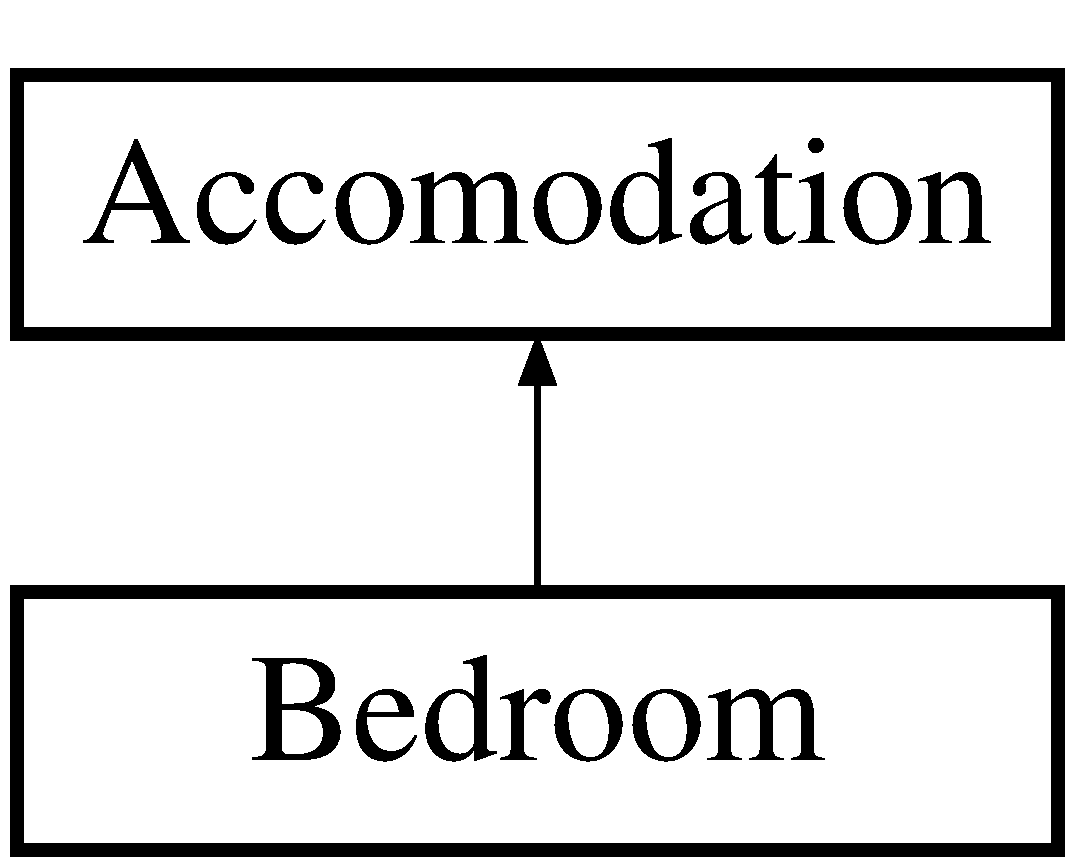
\includegraphics[height=2.000000cm]{class_bedroom}
\end{center}
\end{figure}
\subsection*{Public Member Functions}
\begin{DoxyCompactItemize}
\item 
\hyperlink{class_bedroom_afd743fa0003f9307e4244c22332e1450}{Bedroom} (float price\+\_\+night, float price\+\_\+week, float price\+\_\+month, string location, vector$<$ pair$<$ \hyperlink{class_date}{Date}, \hyperlink{class_date}{Date} $>$$>$ unvailable\+Dates, establishment est, bedroom\+Type bed\+\_\+type)
\begin{DoxyCompactList}\small\item\em bedroom constructor \end{DoxyCompactList}\item 
\hyperlink{class_bedroom_acb17fca3ff7ec73625142fc5360ebfe3}{Bedroom} (unsigned int id, float price\+\_\+night, float price\+\_\+month, float price\+\_\+year, string location, vector$<$ pair$<$ \hyperlink{class_date}{Date}, \hyperlink{class_date}{Date} $>$$>$ unavailable\+Dates, establishment est, bedroom\+Type bed\+\_\+type)
\begin{DoxyCompactList}\small\item\em bedroom constructor with id \end{DoxyCompactList}\item 
\hypertarget{class_bedroom_a227bb14fc225b8c872d85c84163735de}{}\label{class_bedroom_a227bb14fc225b8c872d85c84163735de} 
virtual void \hyperlink{class_bedroom_a227bb14fc225b8c872d85c84163735de}{print} () const
\begin{DoxyCompactList}\small\item\em prints bedroom on the sreen \end{DoxyCompactList}\item 
virtual void \hyperlink{class_bedroom_ad5d0a12fe0257ba5c14efc6182ee33ce}{save\+Accomodation} (ofstream \&out)
\begin{DoxyCompactList}\small\item\em saves bedroom in supliers file \end{DoxyCompactList}\end{DoxyCompactItemize}
\subsection*{Additional Inherited Members}


\subsection{Constructor \& Destructor Documentation}
\hypertarget{class_bedroom_afd743fa0003f9307e4244c22332e1450}{}\label{class_bedroom_afd743fa0003f9307e4244c22332e1450} 
\index{Bedroom@{Bedroom}!Bedroom@{Bedroom}}
\index{Bedroom@{Bedroom}!Bedroom@{Bedroom}}
\subsubsection{\texorpdfstring{Bedroom()}{Bedroom()}\hspace{0.1cm}{\footnotesize\ttfamily [1/2]}}
{\footnotesize\ttfamily Bedroom\+::\+Bedroom (\begin{DoxyParamCaption}\item[{float}]{price\+\_\+night,  }\item[{float}]{price\+\_\+week,  }\item[{float}]{price\+\_\+month,  }\item[{string}]{location,  }\item[{vector$<$ pair$<$ \hyperlink{class_date}{Date}, \hyperlink{class_date}{Date} $>$$>$}]{unvailable\+Dates,  }\item[{establishment}]{est,  }\item[{bedroom\+Type}]{bed\+\_\+type }\end{DoxyParamCaption})}



bedroom constructor 


\begin{DoxyParams}{Parameters}
{\em price\+\_\+night} & \\
\hline
{\em price\+\_\+week} & \\
\hline
{\em price\+\_\+month} & \\
\hline
{\em location} & \\
\hline
{\em unavailable\+\_\+dates} & \\
\hline
{\em est} & type of establishment\\
\hline
{\em bed\+\_\+type} & type of bedroom \\
\hline
\end{DoxyParams}
\hypertarget{class_bedroom_acb17fca3ff7ec73625142fc5360ebfe3}{}\label{class_bedroom_acb17fca3ff7ec73625142fc5360ebfe3} 
\index{Bedroom@{Bedroom}!Bedroom@{Bedroom}}
\index{Bedroom@{Bedroom}!Bedroom@{Bedroom}}
\subsubsection{\texorpdfstring{Bedroom()}{Bedroom()}\hspace{0.1cm}{\footnotesize\ttfamily [2/2]}}
{\footnotesize\ttfamily Bedroom\+::\+Bedroom (\begin{DoxyParamCaption}\item[{unsigned int}]{id,  }\item[{float}]{price\+\_\+night,  }\item[{float}]{price\+\_\+month,  }\item[{float}]{price\+\_\+year,  }\item[{string}]{location,  }\item[{vector$<$ pair$<$ \hyperlink{class_date}{Date}, \hyperlink{class_date}{Date} $>$$>$}]{unavailable\+Dates,  }\item[{establishment}]{est,  }\item[{bedroom\+Type}]{bed\+\_\+type }\end{DoxyParamCaption})}



bedroom constructor with id 


\begin{DoxyParams}{Parameters}
{\em id} & \\
\hline
{\em price\+\_\+night} & \\
\hline
{\em price\+\_\+week} & \\
\hline
{\em price\+\_\+month} & \\
\hline
{\em location} & \\
\hline
{\em unavailable\+\_\+dates} & \\
\hline
{\em est} & type of establishment\\
\hline
{\em bed\+\_\+type} & type of bedroom \\
\hline
\end{DoxyParams}


\subsection{Member Function Documentation}
\hypertarget{class_bedroom_ad5d0a12fe0257ba5c14efc6182ee33ce}{}\label{class_bedroom_ad5d0a12fe0257ba5c14efc6182ee33ce} 
\index{Bedroom@{Bedroom}!save\+Accomodation@{save\+Accomodation}}
\index{save\+Accomodation@{save\+Accomodation}!Bedroom@{Bedroom}}
\subsubsection{\texorpdfstring{save\+Accomodation()}{saveAccomodation()}}
{\footnotesize\ttfamily void Bedroom\+::save\+Accomodation (\begin{DoxyParamCaption}\item[{ofstream \&}]{out }\end{DoxyParamCaption})\hspace{0.3cm}{\ttfamily [virtual]}}



saves bedroom in supliers file 


\begin{DoxyParams}{Parameters}
{\em out} & supliers file \\
\hline
\end{DoxyParams}


Reimplemented from \hyperlink{class_accomodation_a4394eb907b2d5a23faf73dd03c1dac4d}{Accomodation}.



The documentation for this class was generated from the following files\+:\begin{DoxyCompactItemize}
\item 
Accomodation.\+h\item 
Accomodation.\+cpp\end{DoxyCompactItemize}

\hypertarget{class_client}{}\section{Client Class Reference}
\label{class_client}\index{Client@{Client}}
Inheritance diagram for Client\+:\begin{figure}[H]
\begin{center}
\leavevmode
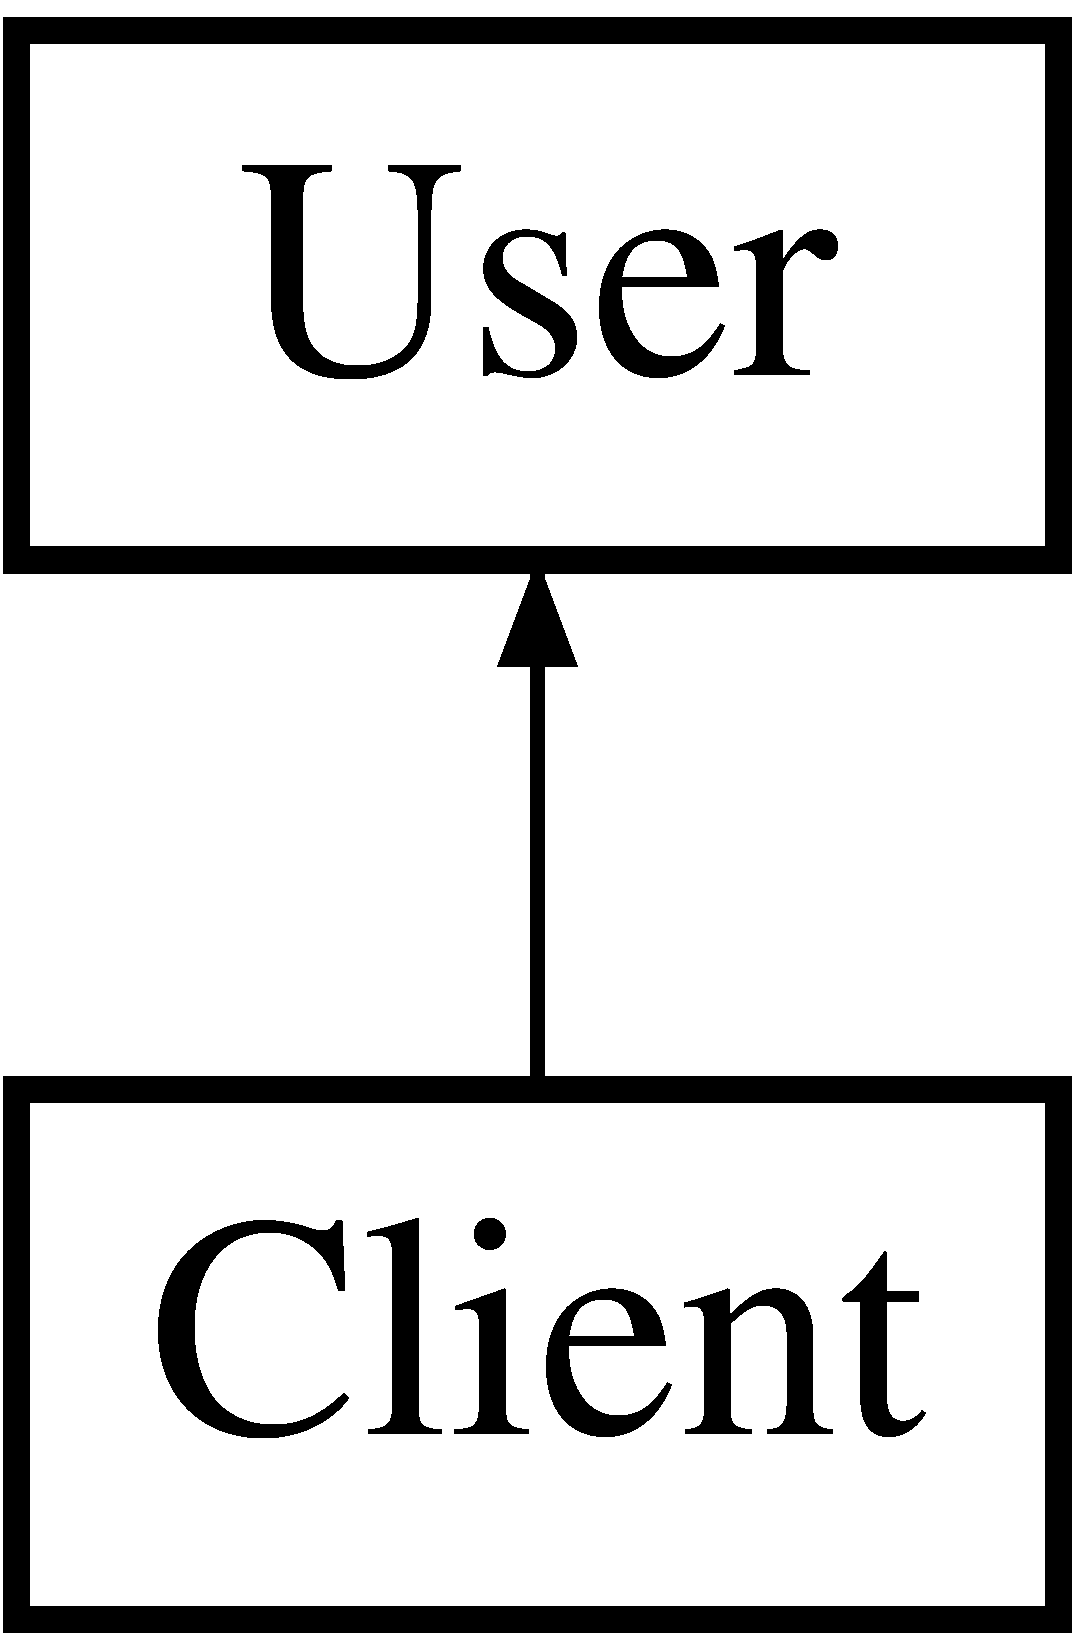
\includegraphics[height=2.000000cm]{class_client}
\end{center}
\end{figure}
\subsection*{Public Member Functions}
\begin{DoxyCompactItemize}
\item 
\hyperlink{class_client_a94e6ab94b8ad2252cc26f3763ec0e253}{Client} (string username, string password, string name, int points=0)
\begin{DoxyCompactList}\small\item\em \hyperlink{class_client}{Client} constructor. \end{DoxyCompactList}\item 
int \hyperlink{class_client_aa3824f589da51dc537ccab1bcfcc8e85}{get\+Points} () const
\begin{DoxyCompactList}\small\item\em gets points \end{DoxyCompactList}\item 
void \hyperlink{class_client_a029f358b9ebb7afbf7ae30e076243b53}{add\+Reservation} (\hyperlink{class_reservation}{Reservation} res)
\begin{DoxyCompactList}\small\item\em adds a reservations to the vector reservations and increments the points based on the price \end{DoxyCompactList}\item 
void \hyperlink{class_client_a2a03ca4558efd182ea5d76dfcec24ecb}{save} (ofstream \&out) const
\begin{DoxyCompactList}\small\item\em saves client uin the file \end{DoxyCompactList}\end{DoxyCompactItemize}


\subsection{Constructor \& Destructor Documentation}
\hypertarget{class_client_a94e6ab94b8ad2252cc26f3763ec0e253}{}\label{class_client_a94e6ab94b8ad2252cc26f3763ec0e253} 
\index{Client@{Client}!Client@{Client}}
\index{Client@{Client}!Client@{Client}}
\subsubsection{\texorpdfstring{Client()}{Client()}}
{\footnotesize\ttfamily Client\+::\+Client (\begin{DoxyParamCaption}\item[{string}]{username,  }\item[{string}]{password,  }\item[{string}]{name,  }\item[{int}]{points = {\ttfamily 0} }\end{DoxyParamCaption})}



\hyperlink{class_client}{Client} constructor. 


\begin{DoxyParams}{Parameters}
{\em username} & \\
\hline
{\em password} & \\
\hline
{\em name} & \\
\hline
{\em points,default} & 0 \\
\hline
\end{DoxyParams}


\subsection{Member Function Documentation}
\hypertarget{class_client_a029f358b9ebb7afbf7ae30e076243b53}{}\label{class_client_a029f358b9ebb7afbf7ae30e076243b53} 
\index{Client@{Client}!add\+Reservation@{add\+Reservation}}
\index{add\+Reservation@{add\+Reservation}!Client@{Client}}
\subsubsection{\texorpdfstring{add\+Reservation()}{addReservation()}}
{\footnotesize\ttfamily void Client\+::add\+Reservation (\begin{DoxyParamCaption}\item[{\hyperlink{class_reservation}{Reservation}}]{res }\end{DoxyParamCaption})}



adds a reservations to the vector reservations and increments the points based on the price 


\begin{DoxyParams}{Parameters}
{\em res} & \\
\hline
\end{DoxyParams}
\hypertarget{class_client_aa3824f589da51dc537ccab1bcfcc8e85}{}\label{class_client_aa3824f589da51dc537ccab1bcfcc8e85} 
\index{Client@{Client}!get\+Points@{get\+Points}}
\index{get\+Points@{get\+Points}!Client@{Client}}
\subsubsection{\texorpdfstring{get\+Points()}{getPoints()}}
{\footnotesize\ttfamily int Client\+::get\+Points (\begin{DoxyParamCaption}{ }\end{DoxyParamCaption}) const\hspace{0.3cm}{\ttfamily [inline]}}



gets points 

\begin{DoxyReturn}{Returns}
po0ints 
\end{DoxyReturn}
\hypertarget{class_client_a2a03ca4558efd182ea5d76dfcec24ecb}{}\label{class_client_a2a03ca4558efd182ea5d76dfcec24ecb} 
\index{Client@{Client}!save@{save}}
\index{save@{save}!Client@{Client}}
\subsubsection{\texorpdfstring{save()}{save()}}
{\footnotesize\ttfamily void Client\+::save (\begin{DoxyParamCaption}\item[{ofstream \&}]{out }\end{DoxyParamCaption}) const}



saves client uin the file 


\begin{DoxyParams}{Parameters}
{\em out} & cleints file \\
\hline
\end{DoxyParams}


The documentation for this class was generated from the following files\+:\begin{DoxyCompactItemize}
\item 
User.\+h\item 
User.\+cpp\end{DoxyCompactItemize}

\hypertarget{class_company}{}\section{Company Class Reference}
\label{class_company}\index{Company@{Company}}
\subsection*{Public Member Functions}
\begin{DoxyCompactItemize}
\item 
\hyperlink{class_company_a50772131ed5edbbcb73bf58dfec71c72}{Company} (string clients\+File, string supliers\+File, string reservations\+File)
\begin{DoxyCompactList}\small\item\em constructor for the \hyperlink{class_company}{Company} based on the files provided \end{DoxyCompactList}\item 
void \hyperlink{class_company_a5a3e5d5ef3ef991c54de2781d0607c19}{supliers\+Inicialization} (string supliers\+File)
\begin{DoxyCompactList}\small\item\em initializes the vector supliers \end{DoxyCompactList}\item 
void \hyperlink{class_company_a79bf900155922f7d8b8b1f248dcc3313}{reservations\+Inicialization} (string reservations\+File)
\begin{DoxyCompactList}\small\item\em initializes the vector reservations and updates the reservations of each suplier \end{DoxyCompactList}\item 
void \hyperlink{class_company_ae2767e861cbe5ddec7111c2d04878c9f}{clients\+Inicialization} (string clients\+File)
\begin{DoxyCompactList}\small\item\em initializes the vector of clients \end{DoxyCompactList}\item 
\hypertarget{class_company_af124ca1bb17d8450ab129a33a5f8d4be}{}\label{class_company_af124ca1bb17d8450ab129a33a5f8d4be} 
void \hyperlink{class_company_af124ca1bb17d8450ab129a33a5f8d4be}{register\+Suplier} ()
\begin{DoxyCompactList}\small\item\em handles the registantion of a suplier \end{DoxyCompactList}\item 
\hypertarget{class_company_a402904c6651146a9ca6023e72bd6c8fc}{}\label{class_company_a402904c6651146a9ca6023e72bd6c8fc} 
void \hyperlink{class_company_a402904c6651146a9ca6023e72bd6c8fc}{register\+Client} ()
\begin{DoxyCompactList}\small\item\em handles the registantion of a client \end{DoxyCompactList}\item 
vector$<$ \hyperlink{class_suplier}{Suplier} $>$\+::iterator \hyperlink{class_company_a9012e0fa84141868a482a0a69b6313af}{verify\+Log\+In\+Sup} (string username, string password)
\begin{DoxyCompactList}\small\item\em verifies if the username and password of a suplier are correct \end{DoxyCompactList}\item 
vector$<$ \hyperlink{class_client}{Client} $>$\+::iterator \hyperlink{class_company_ae09dab4c6a0d26207cdeffd0d5adcf8f}{verify\+Log\+In\+Cli} (string username, string password)
\begin{DoxyCompactList}\small\item\em verifies if the username and password of a client are correct \end{DoxyCompactList}\item 
\hyperlink{class_accomodation}{Accomodation} $\ast$ \hyperlink{class_company_a2b6d438df8e871898eef5fc5e3e8f761}{display\+Offers} (string location, \hyperlink{class_date}{Date} initial\+\_\+date, \hyperlink{class_date}{Date} final\+\_\+\+Date)
\begin{DoxyCompactList}\small\item\em display the accomodations that correspond to the restrictions given by the client and asks him to choose onde of them \end{DoxyCompactList}\item 
void \hyperlink{class_company_aafc4b607edcf5a01500c42c03d1322ad}{add\+Reservation\+Comp} (\hyperlink{class_accomodation}{Accomodation} $\ast$a, \hyperlink{class_date}{Date} init\+\_\+date, \hyperlink{class_date}{Date} final\+\_\+date)
\begin{DoxyCompactList}\small\item\em adds a reservations to the reservations vector and to the suplier that owns tha accomodation a \end{DoxyCompactList}\item 
int \hyperlink{class_company_ab3dbac165de998e1e711a6dba7cbbf51}{cancel\+Reservation} ()
\begin{DoxyCompactList}\small\item\em ask the client wich reservation he wants to to cancel removes it from the vectors and displays the amount that the client must receive \end{DoxyCompactList}\item 
\hypertarget{class_company_aec3da42cd9c40660c9b6478dfb246109}{}\label{class_company_aec3da42cd9c40660c9b6478dfb246109} 
void \hyperlink{class_company_aec3da42cd9c40660c9b6478dfb246109}{show\+Reservation} () const
\begin{DoxyCompactList}\small\item\em asks for the id of the reservation and displays it on the screen \end{DoxyCompactList}\item 
\hypertarget{class_company_a72134cd31bcd5a1bac08ad8e6235d28f}{}\label{class_company_a72134cd31bcd5a1bac08ad8e6235d28f} 
void \hyperlink{class_company_a72134cd31bcd5a1bac08ad8e6235d28f}{save\+Changes} () const
\begin{DoxyCompactList}\small\item\em saves changes of supliers, clients and reservations on the respective files \end{DoxyCompactList}\item 
\hypertarget{class_company_ae5cc3089ac58af98b1f4a0b3a7d7e7af}{}\label{class_company_ae5cc3089ac58af98b1f4a0b3a7d7e7af} 
void \hyperlink{class_company_ae5cc3089ac58af98b1f4a0b3a7d7e7af}{save\+Clients\+Changes} () const
\begin{DoxyCompactList}\small\item\em saves changes in clients file \end{DoxyCompactList}\item 
\hypertarget{class_company_a0c8230826db8ef8884e06e0fba61800e}{}\label{class_company_a0c8230826db8ef8884e06e0fba61800e} 
void \hyperlink{class_company_a0c8230826db8ef8884e06e0fba61800e}{save\+Supliers\+Changes} () const
\begin{DoxyCompactList}\small\item\em saves changes in supliers file \end{DoxyCompactList}\item 
\hypertarget{class_company_ad9a63c107f1d1c763577961e42aae6c8}{}\label{class_company_ad9a63c107f1d1c763577961e42aae6c8} 
void \hyperlink{class_company_ad9a63c107f1d1c763577961e42aae6c8}{save\+Reservations\+Changes} () const
\begin{DoxyCompactList}\small\item\em saves changes in reservtaions file \end{DoxyCompactList}\end{DoxyCompactItemize}


\subsection{Constructor \& Destructor Documentation}
\hypertarget{class_company_a50772131ed5edbbcb73bf58dfec71c72}{}\label{class_company_a50772131ed5edbbcb73bf58dfec71c72} 
\index{Company@{Company}!Company@{Company}}
\index{Company@{Company}!Company@{Company}}
\subsubsection{\texorpdfstring{Company()}{Company()}}
{\footnotesize\ttfamily Company\+::\+Company (\begin{DoxyParamCaption}\item[{string}]{clients\+File,  }\item[{string}]{supliers\+File,  }\item[{string}]{reservations\+File }\end{DoxyParamCaption})}



constructor for the \hyperlink{class_company}{Company} based on the files provided 


\begin{DoxyParams}{Parameters}
{\em clients\+File} & file of clients\\
\hline
{\em supliers\+File} & file of supliers\\
\hline
{\em revervations\+File} & file of reservations \\
\hline
\end{DoxyParams}


\subsection{Member Function Documentation}
\hypertarget{class_company_aafc4b607edcf5a01500c42c03d1322ad}{}\label{class_company_aafc4b607edcf5a01500c42c03d1322ad} 
\index{Company@{Company}!add\+Reservation\+Comp@{add\+Reservation\+Comp}}
\index{add\+Reservation\+Comp@{add\+Reservation\+Comp}!Company@{Company}}
\subsubsection{\texorpdfstring{add\+Reservation\+Comp()}{addReservationComp()}}
{\footnotesize\ttfamily void Company\+::add\+Reservation\+Comp (\begin{DoxyParamCaption}\item[{\hyperlink{class_accomodation}{Accomodation} $\ast$}]{a,  }\item[{\hyperlink{class_date}{Date}}]{init\+\_\+date,  }\item[{\hyperlink{class_date}{Date}}]{final\+\_\+date }\end{DoxyParamCaption})}



adds a reservations to the reservations vector and to the suplier that owns tha accomodation a 


\begin{DoxyParams}{Parameters}
{\em a} & accomodation linked to the reservation to add\\
\hline
{\em init\+\_\+date} & check in date\\
\hline
{\em final\+\_\+date} & check out date \\
\hline
\end{DoxyParams}
\hypertarget{class_company_ab3dbac165de998e1e711a6dba7cbbf51}{}\label{class_company_ab3dbac165de998e1e711a6dba7cbbf51} 
\index{Company@{Company}!cancel\+Reservation@{cancel\+Reservation}}
\index{cancel\+Reservation@{cancel\+Reservation}!Company@{Company}}
\subsubsection{\texorpdfstring{cancel\+Reservation()}{cancelReservation()}}
{\footnotesize\ttfamily int Company\+::cancel\+Reservation (\begin{DoxyParamCaption}{ }\end{DoxyParamCaption})}



ask the client wich reservation he wants to to cancel removes it from the vectors and displays the amount that the client must receive 

\begin{DoxyReturn}{Returns}
id of the reservation deleeted 
\end{DoxyReturn}
\hypertarget{class_company_ae2767e861cbe5ddec7111c2d04878c9f}{}\label{class_company_ae2767e861cbe5ddec7111c2d04878c9f} 
\index{Company@{Company}!clients\+Inicialization@{clients\+Inicialization}}
\index{clients\+Inicialization@{clients\+Inicialization}!Company@{Company}}
\subsubsection{\texorpdfstring{clients\+Inicialization()}{clientsInicialization()}}
{\footnotesize\ttfamily void Company\+::clients\+Inicialization (\begin{DoxyParamCaption}\item[{string}]{clients\+File }\end{DoxyParamCaption})}



initializes the vector of clients 


\begin{DoxyParams}{Parameters}
{\em clients\+File} & file of clients \\
\hline
\end{DoxyParams}
\hypertarget{class_company_a2b6d438df8e871898eef5fc5e3e8f761}{}\label{class_company_a2b6d438df8e871898eef5fc5e3e8f761} 
\index{Company@{Company}!display\+Offers@{display\+Offers}}
\index{display\+Offers@{display\+Offers}!Company@{Company}}
\subsubsection{\texorpdfstring{display\+Offers()}{displayOffers()}}
{\footnotesize\ttfamily \hyperlink{class_accomodation}{Accomodation} $\ast$ Company\+::display\+Offers (\begin{DoxyParamCaption}\item[{string}]{location,  }\item[{\hyperlink{class_date}{Date}}]{initial\+\_\+date,  }\item[{\hyperlink{class_date}{Date}}]{final\+\_\+\+Date }\end{DoxyParamCaption})}



display the accomodations that correspond to the restrictions given by the client and asks him to choose onde of them 


\begin{DoxyParams}{Parameters}
{\em location} & location of the accomodations that must be displayed\\
\hline
{\em initial\+\_\+date} & check in date\\
\hline
{\em final\+\_\+date} & check out date\\
\hline
\end{DoxyParams}
\begin{DoxyReturn}{Returns}
pointer to the accomodation chooe by the client or N\+U\+LL pointer if there is no accomodation that respect the restrictions or if the id that the client chose does no exist 
\end{DoxyReturn}
\hypertarget{class_company_a79bf900155922f7d8b8b1f248dcc3313}{}\label{class_company_a79bf900155922f7d8b8b1f248dcc3313} 
\index{Company@{Company}!reservations\+Inicialization@{reservations\+Inicialization}}
\index{reservations\+Inicialization@{reservations\+Inicialization}!Company@{Company}}
\subsubsection{\texorpdfstring{reservations\+Inicialization()}{reservationsInicialization()}}
{\footnotesize\ttfamily void Company\+::reservations\+Inicialization (\begin{DoxyParamCaption}\item[{string}]{reservations\+File }\end{DoxyParamCaption})}



initializes the vector reservations and updates the reservations of each suplier 


\begin{DoxyParams}{Parameters}
{\em reservations\+File} & file of reservations \\
\hline
\end{DoxyParams}
\hypertarget{class_company_a5a3e5d5ef3ef991c54de2781d0607c19}{}\label{class_company_a5a3e5d5ef3ef991c54de2781d0607c19} 
\index{Company@{Company}!supliers\+Inicialization@{supliers\+Inicialization}}
\index{supliers\+Inicialization@{supliers\+Inicialization}!Company@{Company}}
\subsubsection{\texorpdfstring{supliers\+Inicialization()}{supliersInicialization()}}
{\footnotesize\ttfamily void Company\+::supliers\+Inicialization (\begin{DoxyParamCaption}\item[{string}]{supliers\+File }\end{DoxyParamCaption})}



initializes the vector supliers 


\begin{DoxyParams}{Parameters}
{\em supliers\+File} & file of supliers \\
\hline
\end{DoxyParams}
\hypertarget{class_company_ae09dab4c6a0d26207cdeffd0d5adcf8f}{}\label{class_company_ae09dab4c6a0d26207cdeffd0d5adcf8f} 
\index{Company@{Company}!verify\+Log\+In\+Cli@{verify\+Log\+In\+Cli}}
\index{verify\+Log\+In\+Cli@{verify\+Log\+In\+Cli}!Company@{Company}}
\subsubsection{\texorpdfstring{verify\+Log\+In\+Cli()}{verifyLogInCli()}}
{\footnotesize\ttfamily vector$<$ \hyperlink{class_client}{Client} $>$\+::iterator Company\+::verify\+Log\+In\+Cli (\begin{DoxyParamCaption}\item[{string}]{username,  }\item[{string}]{password }\end{DoxyParamCaption})}



verifies if the username and password of a client are correct 


\begin{DoxyParams}{Parameters}
{\em username} & username of the client\\
\hline
{\em password} & password of the client\\
\hline
\end{DoxyParams}
\begin{DoxyReturn}{Returns}
iterator for the client with the username and password given 
\end{DoxyReturn}
\hypertarget{class_company_a9012e0fa84141868a482a0a69b6313af}{}\label{class_company_a9012e0fa84141868a482a0a69b6313af} 
\index{Company@{Company}!verify\+Log\+In\+Sup@{verify\+Log\+In\+Sup}}
\index{verify\+Log\+In\+Sup@{verify\+Log\+In\+Sup}!Company@{Company}}
\subsubsection{\texorpdfstring{verify\+Log\+In\+Sup()}{verifyLogInSup()}}
{\footnotesize\ttfamily vector$<$ \hyperlink{class_suplier}{Suplier} $>$\+::iterator Company\+::verify\+Log\+In\+Sup (\begin{DoxyParamCaption}\item[{string}]{username,  }\item[{string}]{password }\end{DoxyParamCaption})}



verifies if the username and password of a suplier are correct 


\begin{DoxyParams}{Parameters}
{\em username} & username of the suplier\\
\hline
{\em password} & password of the suplier\\
\hline
\end{DoxyParams}
\begin{DoxyReturn}{Returns}
iterator for the suplier with the username and password given 
\end{DoxyReturn}


The documentation for this class was generated from the following files\+:\begin{DoxyCompactItemize}
\item 
Company.\+h\item 
Company.\+cpp\end{DoxyCompactItemize}

\hypertarget{class_date}{}\section{Date Class Reference}
\label{class_date}\index{Date@{Date}}
\subsection*{Public Member Functions}
\begin{DoxyCompactItemize}
\item 
\hyperlink{class_date_a5532efafed41fd5f8e013a61313200dc}{Date} (string date)
\begin{DoxyCompactList}\small\item\em date constructor \end{DoxyCompactList}\item 
int \hyperlink{class_date_a0f253815240e70f4c39cb93cc68bd3f4}{get\+Day} () const
\begin{DoxyCompactList}\small\item\em gets day \end{DoxyCompactList}\item 
int \hyperlink{class_date_a332f6e3a2f6a40d73742b6dab7be0f64}{get\+Month} () const
\begin{DoxyCompactList}\small\item\em gets month \end{DoxyCompactList}\item 
int \hyperlink{class_date_a8b0869f34c2b38d108ab83ee2e770e5d}{get\+Year} () const
\begin{DoxyCompactList}\small\item\em gets year \end{DoxyCompactList}\item 
void \hyperlink{class_date_a2f97b9d1ac5ef0ef6b6cab3335c5303d}{set\+Day} (int day)
\begin{DoxyCompactList}\small\item\em sets day \end{DoxyCompactList}\item 
void \hyperlink{class_date_a23aa56014dd581d691607df5d4474f64}{set\+Month} (int month)
\begin{DoxyCompactList}\small\item\em sets month \end{DoxyCompactList}\item 
void \hyperlink{class_date_a895c4ae9868e43577cf59d9c679d7a71}{set\+Year} (int year)
\begin{DoxyCompactList}\small\item\em sets year \end{DoxyCompactList}\item 
int \hyperlink{class_date_a8e10a688e6056a4d62a8c5ba5de11e54}{convert\+\_\+date\+\_\+int} () const
\begin{DoxyCompactList}\small\item\em converts date into an integer \end{DoxyCompactList}\item 
bool \hyperlink{class_date_ac44b1159cfc6b4936fddd909b0c2a8f1}{leap\+Year} (int year)
\begin{DoxyCompactList}\small\item\em checks if year is leap \end{DoxyCompactList}\item 
bool \hyperlink{class_date_ab068a7017e7033adba1680de395c844e}{is\+Leap} (int year)
\begin{DoxyCompactList}\small\item\em checks if year is leap \end{DoxyCompactList}\item 
bool \hyperlink{class_date_ac4810ddec014ca51257871abac9667a9}{check\+Date} ()
\begin{DoxyCompactList}\small\item\em checks if date is valid \end{DoxyCompactList}\item 
bool \hyperlink{class_date_a5693be8bccd3d4bd431a2cb0ae042d02}{get\+Date} (string date\+\_\+str)
\begin{DoxyCompactList}\small\item\em checks if date is valid and correctly extracted \end{DoxyCompactList}\end{DoxyCompactItemize}
\subsection*{Friends}
\begin{DoxyCompactItemize}
\item 
bool \hyperlink{class_date_a9aae61020a07731a50cc80927fd8d346}{operator$>$=} (const \hyperlink{class_date}{Date} \&d1, const \hyperlink{class_date}{Date} \&d2)
\begin{DoxyCompactList}\small\item\em checks if d1 is higher or equal to d2 \end{DoxyCompactList}\item 
bool \hyperlink{class_date_a4f314b2216e8760eac284385a7eaae12}{operator$<$=} (const \hyperlink{class_date}{Date} \&d1, const \hyperlink{class_date}{Date} \&d2)
\begin{DoxyCompactList}\small\item\em checks if d1 is less or equal to d2 \end{DoxyCompactList}\item 
bool \hyperlink{class_date_a5a3f411cbd59e9ecb90b2f8e6aaea551}{operator$<$} (const \hyperlink{class_date}{Date} \&d1, const \hyperlink{class_date}{Date} \&d2)
\begin{DoxyCompactList}\small\item\em checks if d1 is less than d2 \end{DoxyCompactList}\item 
bool \hyperlink{class_date_a5c40ea6f65fef5d3e1ed8bec5e16ec41}{operator$>$} (const \hyperlink{class_date}{Date} \&d1, const \hyperlink{class_date}{Date} \&d2)
\begin{DoxyCompactList}\small\item\em checks if d1 is higher than d2 \end{DoxyCompactList}\item 
bool \hyperlink{class_date_a18dc8aca1ca4d8cadc2b464db984135b}{operator==} (const \hyperlink{class_date}{Date} \&d1, const \hyperlink{class_date}{Date} \&d2)
\begin{DoxyCompactList}\small\item\em checks if d1 is equal to d2 \end{DoxyCompactList}\item 
ostream \& \hyperlink{class_date_a5c29d00ecf33e6d232a410f1f3d6eb70}{operator$<$$<$} (ostream \&out, const \hyperlink{class_date}{Date} \&date)
\begin{DoxyCompactList}\small\item\em displays date \end{DoxyCompactList}\end{DoxyCompactItemize}


\subsection{Constructor \& Destructor Documentation}
\hypertarget{class_date_a5532efafed41fd5f8e013a61313200dc}{}\label{class_date_a5532efafed41fd5f8e013a61313200dc} 
\index{Date@{Date}!Date@{Date}}
\index{Date@{Date}!Date@{Date}}
\subsubsection{\texorpdfstring{Date()}{Date()}}
{\footnotesize\ttfamily Date\+::\+Date (\begin{DoxyParamCaption}\item[{string}]{date }\end{DoxyParamCaption})}



date constructor 


\begin{DoxyParams}{Parameters}
{\em date} & in D\+D/\+M\+M/\+Y\+Y\+YY format \\
\hline
\end{DoxyParams}


\subsection{Member Function Documentation}
\hypertarget{class_date_ac4810ddec014ca51257871abac9667a9}{}\label{class_date_ac4810ddec014ca51257871abac9667a9} 
\index{Date@{Date}!check\+Date@{check\+Date}}
\index{check\+Date@{check\+Date}!Date@{Date}}
\subsubsection{\texorpdfstring{check\+Date()}{checkDate()}}
{\footnotesize\ttfamily bool Date\+::check\+Date (\begin{DoxyParamCaption}{ }\end{DoxyParamCaption})}



checks if date is valid 

\begin{DoxyReturn}{Returns}
true if valid, false otherwise 
\end{DoxyReturn}
\hypertarget{class_date_a8e10a688e6056a4d62a8c5ba5de11e54}{}\label{class_date_a8e10a688e6056a4d62a8c5ba5de11e54} 
\index{Date@{Date}!convert\+\_\+date\+\_\+int@{convert\+\_\+date\+\_\+int}}
\index{convert\+\_\+date\+\_\+int@{convert\+\_\+date\+\_\+int}!Date@{Date}}
\subsubsection{\texorpdfstring{convert\+\_\+date\+\_\+int()}{convert\_date\_int()}}
{\footnotesize\ttfamily int Date\+::convert\+\_\+date\+\_\+int (\begin{DoxyParamCaption}{ }\end{DoxyParamCaption}) const}



converts date into an integer 

\begin{DoxyReturn}{Returns}
integer corresponding to date 
\end{DoxyReturn}
\hypertarget{class_date_a5693be8bccd3d4bd431a2cb0ae042d02}{}\label{class_date_a5693be8bccd3d4bd431a2cb0ae042d02} 
\index{Date@{Date}!get\+Date@{get\+Date}}
\index{get\+Date@{get\+Date}!Date@{Date}}
\subsubsection{\texorpdfstring{get\+Date()}{getDate()}}
{\footnotesize\ttfamily bool Date\+::get\+Date (\begin{DoxyParamCaption}\item[{string}]{date\+\_\+str }\end{DoxyParamCaption})}



checks if date is valid and correctly extracted 


\begin{DoxyParams}{Parameters}
{\em date\+\_\+str} & \\
\hline
\end{DoxyParams}
\begin{DoxyReturn}{Returns}
true if valid, false otherwise 
\end{DoxyReturn}
\hypertarget{class_date_a0f253815240e70f4c39cb93cc68bd3f4}{}\label{class_date_a0f253815240e70f4c39cb93cc68bd3f4} 
\index{Date@{Date}!get\+Day@{get\+Day}}
\index{get\+Day@{get\+Day}!Date@{Date}}
\subsubsection{\texorpdfstring{get\+Day()}{getDay()}}
{\footnotesize\ttfamily int Date\+::get\+Day (\begin{DoxyParamCaption}{ }\end{DoxyParamCaption}) const}



gets day 

\begin{DoxyReturn}{Returns}
day 
\end{DoxyReturn}
\hypertarget{class_date_a332f6e3a2f6a40d73742b6dab7be0f64}{}\label{class_date_a332f6e3a2f6a40d73742b6dab7be0f64} 
\index{Date@{Date}!get\+Month@{get\+Month}}
\index{get\+Month@{get\+Month}!Date@{Date}}
\subsubsection{\texorpdfstring{get\+Month()}{getMonth()}}
{\footnotesize\ttfamily int Date\+::get\+Month (\begin{DoxyParamCaption}{ }\end{DoxyParamCaption}) const}



gets month 

\begin{DoxyReturn}{Returns}
month 
\end{DoxyReturn}
\hypertarget{class_date_a8b0869f34c2b38d108ab83ee2e770e5d}{}\label{class_date_a8b0869f34c2b38d108ab83ee2e770e5d} 
\index{Date@{Date}!get\+Year@{get\+Year}}
\index{get\+Year@{get\+Year}!Date@{Date}}
\subsubsection{\texorpdfstring{get\+Year()}{getYear()}}
{\footnotesize\ttfamily int Date\+::get\+Year (\begin{DoxyParamCaption}{ }\end{DoxyParamCaption}) const}



gets year 

\begin{DoxyReturn}{Returns}
year 
\end{DoxyReturn}
\hypertarget{class_date_ab068a7017e7033adba1680de395c844e}{}\label{class_date_ab068a7017e7033adba1680de395c844e} 
\index{Date@{Date}!is\+Leap@{is\+Leap}}
\index{is\+Leap@{is\+Leap}!Date@{Date}}
\subsubsection{\texorpdfstring{is\+Leap()}{isLeap()}}
{\footnotesize\ttfamily bool Date\+::is\+Leap (\begin{DoxyParamCaption}\item[{int}]{year }\end{DoxyParamCaption})}



checks if year is leap 


\begin{DoxyParams}{Parameters}
{\em year} & \\
\hline
\end{DoxyParams}
\begin{DoxyReturn}{Returns}
true if leap, false otherwise 
\end{DoxyReturn}
\hypertarget{class_date_ac44b1159cfc6b4936fddd909b0c2a8f1}{}\label{class_date_ac44b1159cfc6b4936fddd909b0c2a8f1} 
\index{Date@{Date}!leap\+Year@{leap\+Year}}
\index{leap\+Year@{leap\+Year}!Date@{Date}}
\subsubsection{\texorpdfstring{leap\+Year()}{leapYear()}}
{\footnotesize\ttfamily bool Date\+::leap\+Year (\begin{DoxyParamCaption}\item[{int}]{year }\end{DoxyParamCaption})}



checks if year is leap 


\begin{DoxyParams}{Parameters}
{\em year} & \\
\hline
\end{DoxyParams}
\begin{DoxyReturn}{Returns}
true if leap, false otherwise 
\end{DoxyReturn}
\hypertarget{class_date_a2f97b9d1ac5ef0ef6b6cab3335c5303d}{}\label{class_date_a2f97b9d1ac5ef0ef6b6cab3335c5303d} 
\index{Date@{Date}!set\+Day@{set\+Day}}
\index{set\+Day@{set\+Day}!Date@{Date}}
\subsubsection{\texorpdfstring{set\+Day()}{setDay()}}
{\footnotesize\ttfamily void Date\+::set\+Day (\begin{DoxyParamCaption}\item[{int}]{day }\end{DoxyParamCaption})}



sets day 


\begin{DoxyParams}{Parameters}
{\em day} & \\
\hline
\end{DoxyParams}
\hypertarget{class_date_a23aa56014dd581d691607df5d4474f64}{}\label{class_date_a23aa56014dd581d691607df5d4474f64} 
\index{Date@{Date}!set\+Month@{set\+Month}}
\index{set\+Month@{set\+Month}!Date@{Date}}
\subsubsection{\texorpdfstring{set\+Month()}{setMonth()}}
{\footnotesize\ttfamily void Date\+::set\+Month (\begin{DoxyParamCaption}\item[{int}]{month }\end{DoxyParamCaption})}



sets month 


\begin{DoxyParams}{Parameters}
{\em mont} & \\
\hline
\end{DoxyParams}
\hypertarget{class_date_a895c4ae9868e43577cf59d9c679d7a71}{}\label{class_date_a895c4ae9868e43577cf59d9c679d7a71} 
\index{Date@{Date}!set\+Year@{set\+Year}}
\index{set\+Year@{set\+Year}!Date@{Date}}
\subsubsection{\texorpdfstring{set\+Year()}{setYear()}}
{\footnotesize\ttfamily void Date\+::set\+Year (\begin{DoxyParamCaption}\item[{int}]{year }\end{DoxyParamCaption})}



sets year 


\begin{DoxyParams}{Parameters}
{\em year} & \\
\hline
\end{DoxyParams}


\subsection{Friends And Related Function Documentation}
\hypertarget{class_date_a5a3f411cbd59e9ecb90b2f8e6aaea551}{}\label{class_date_a5a3f411cbd59e9ecb90b2f8e6aaea551} 
\index{Date@{Date}!operator$<$@{operator$<$}}
\index{operator$<$@{operator$<$}!Date@{Date}}
\subsubsection{\texorpdfstring{operator$<$}{operator<}}
{\footnotesize\ttfamily bool operator$<$ (\begin{DoxyParamCaption}\item[{const \hyperlink{class_date}{Date} \&}]{d1,  }\item[{const \hyperlink{class_date}{Date} \&}]{d2 }\end{DoxyParamCaption})\hspace{0.3cm}{\ttfamily [friend]}}



checks if d1 is less than d2 


\begin{DoxyParams}{Parameters}
{\em d1} & \\
\hline
{\em d2} & \\
\hline
\end{DoxyParams}
\begin{DoxyReturn}{Returns}
true if d1 is less than d2, false otherwise 
\end{DoxyReturn}
\hypertarget{class_date_a5c29d00ecf33e6d232a410f1f3d6eb70}{}\label{class_date_a5c29d00ecf33e6d232a410f1f3d6eb70} 
\index{Date@{Date}!operator$<$$<$@{operator$<$$<$}}
\index{operator$<$$<$@{operator$<$$<$}!Date@{Date}}
\subsubsection{\texorpdfstring{operator$<$$<$}{operator<<}}
{\footnotesize\ttfamily ostream\& operator$<$$<$ (\begin{DoxyParamCaption}\item[{ostream \&}]{out,  }\item[{const \hyperlink{class_date}{Date} \&}]{date }\end{DoxyParamCaption})\hspace{0.3cm}{\ttfamily [friend]}}



displays date 


\begin{DoxyParams}{Parameters}
{\em out} & \\
\hline
{\em date} & \\
\hline
\end{DoxyParams}
\begin{DoxyReturn}{Returns}
out 
\end{DoxyReturn}
\hypertarget{class_date_a4f314b2216e8760eac284385a7eaae12}{}\label{class_date_a4f314b2216e8760eac284385a7eaae12} 
\index{Date@{Date}!operator$<$=@{operator$<$=}}
\index{operator$<$=@{operator$<$=}!Date@{Date}}
\subsubsection{\texorpdfstring{operator$<$=}{operator<=}}
{\footnotesize\ttfamily bool operator$<$= (\begin{DoxyParamCaption}\item[{const \hyperlink{class_date}{Date} \&}]{d1,  }\item[{const \hyperlink{class_date}{Date} \&}]{d2 }\end{DoxyParamCaption})\hspace{0.3cm}{\ttfamily [friend]}}



checks if d1 is less or equal to d2 


\begin{DoxyParams}{Parameters}
{\em d1} & \\
\hline
{\em d2} & \\
\hline
\end{DoxyParams}
\begin{DoxyReturn}{Returns}
true if d1 is less or equal to d2, false otherwise 
\end{DoxyReturn}
\hypertarget{class_date_a18dc8aca1ca4d8cadc2b464db984135b}{}\label{class_date_a18dc8aca1ca4d8cadc2b464db984135b} 
\index{Date@{Date}!operator==@{operator==}}
\index{operator==@{operator==}!Date@{Date}}
\subsubsection{\texorpdfstring{operator==}{operator==}}
{\footnotesize\ttfamily bool operator== (\begin{DoxyParamCaption}\item[{const \hyperlink{class_date}{Date} \&}]{d1,  }\item[{const \hyperlink{class_date}{Date} \&}]{d2 }\end{DoxyParamCaption})\hspace{0.3cm}{\ttfamily [friend]}}



checks if d1 is equal to d2 


\begin{DoxyParams}{Parameters}
{\em d1} & \\
\hline
{\em d2} & \\
\hline
\end{DoxyParams}
\begin{DoxyReturn}{Returns}
true if d1 is equal to d2, false otherwise 
\end{DoxyReturn}
\hypertarget{class_date_a5c40ea6f65fef5d3e1ed8bec5e16ec41}{}\label{class_date_a5c40ea6f65fef5d3e1ed8bec5e16ec41} 
\index{Date@{Date}!operator$>$@{operator$>$}}
\index{operator$>$@{operator$>$}!Date@{Date}}
\subsubsection{\texorpdfstring{operator$>$}{operator>}}
{\footnotesize\ttfamily bool operator$>$ (\begin{DoxyParamCaption}\item[{const \hyperlink{class_date}{Date} \&}]{d1,  }\item[{const \hyperlink{class_date}{Date} \&}]{d2 }\end{DoxyParamCaption})\hspace{0.3cm}{\ttfamily [friend]}}



checks if d1 is higher than d2 


\begin{DoxyParams}{Parameters}
{\em d1} & \\
\hline
{\em d2} & \\
\hline
\end{DoxyParams}
\begin{DoxyReturn}{Returns}
true if d1 is higher than d2, false otherwise 
\end{DoxyReturn}
\hypertarget{class_date_a9aae61020a07731a50cc80927fd8d346}{}\label{class_date_a9aae61020a07731a50cc80927fd8d346} 
\index{Date@{Date}!operator$>$=@{operator$>$=}}
\index{operator$>$=@{operator$>$=}!Date@{Date}}
\subsubsection{\texorpdfstring{operator$>$=}{operator>=}}
{\footnotesize\ttfamily bool operator$>$= (\begin{DoxyParamCaption}\item[{const \hyperlink{class_date}{Date} \&}]{d1,  }\item[{const \hyperlink{class_date}{Date} \&}]{d2 }\end{DoxyParamCaption})\hspace{0.3cm}{\ttfamily [friend]}}



checks if d1 is higher or equal to d2 


\begin{DoxyParams}{Parameters}
{\em d1} & \\
\hline
{\em d2} & \\
\hline
\end{DoxyParams}
\begin{DoxyReturn}{Returns}
true if d1 is higher or equal to d2, false otherwise 
\end{DoxyReturn}


The documentation for this class was generated from the following files\+:\begin{DoxyCompactItemize}
\item 
Date.\+h\item 
Date.\+cpp\end{DoxyCompactItemize}

\hypertarget{class_error_opening_file}{}\section{Error\+Opening\+File Class Reference}
\label{class_error_opening_file}\index{Error\+Opening\+File@{Error\+Opening\+File}}
\subsection*{Public Member Functions}
\begin{DoxyCompactItemize}
\item 
\hypertarget{class_error_opening_file_a1e5ab065abd8e5cfa827730f9e9b06d4}{}\label{class_error_opening_file_a1e5ab065abd8e5cfa827730f9e9b06d4} 
{\bfseries Error\+Opening\+File} (string file\+\_\+type)
\end{DoxyCompactItemize}
\subsection*{Friends}
\begin{DoxyCompactItemize}
\item 
\hypertarget{class_error_opening_file_af72ed5066b7bbfc4485454291cb5356c}{}\label{class_error_opening_file_af72ed5066b7bbfc4485454291cb5356c} 
ostream \& {\bfseries operator$<$$<$} (ostream \&out, \hyperlink{class_error_opening_file}{Error\+Opening\+File} \&eof)
\end{DoxyCompactItemize}


The documentation for this class was generated from the following file\+:\begin{DoxyCompactItemize}
\item 
utils.\+h\end{DoxyCompactItemize}

\hypertarget{class_flat}{}\section{Flat Class Reference}
\label{class_flat}\index{Flat@{Flat}}
Inheritance diagram for Flat\+:\begin{figure}[H]
\begin{center}
\leavevmode
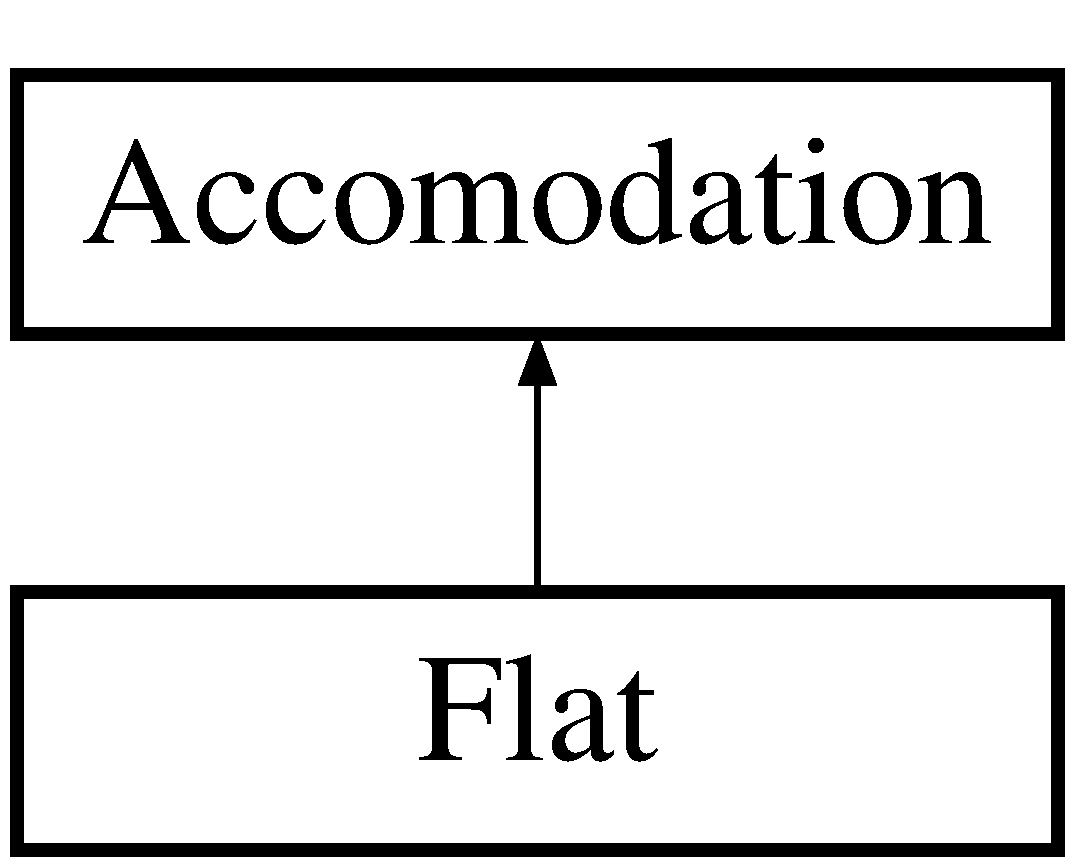
\includegraphics[height=2.000000cm]{class_flat}
\end{center}
\end{figure}
\subsection*{Public Member Functions}
\begin{DoxyCompactItemize}
\item 
\hyperlink{class_flat_afa99056abbef313ebb20cdf4cc66bd14}{Flat} (float price\+\_\+night, float price\+\_\+week, float price\+\_\+month, string location, vector$<$ pair$<$ \hyperlink{class_date}{Date}, \hyperlink{class_date}{Date} $>$$>$ unavailable\+Dates)
\begin{DoxyCompactList}\small\item\em flat constructor \end{DoxyCompactList}\item 
\hyperlink{class_flat_a9ae64f076ea0fd8d191cedb5bda50e39}{Flat} (unsigned int id, float price\+\_\+night, float price\+\_\+week, float price\+\_\+month, string location, vector$<$ pair$<$ \hyperlink{class_date}{Date}, \hyperlink{class_date}{Date} $>$$>$ unavailable\+Dates)
\begin{DoxyCompactList}\small\item\em flat constructor with id \end{DoxyCompactList}\item 
\hypertarget{class_flat_a9ba466cf178ef918f571145838d81173}{}\label{class_flat_a9ba466cf178ef918f571145838d81173} 
virtual void \hyperlink{class_flat_a9ba466cf178ef918f571145838d81173}{print} () const
\begin{DoxyCompactList}\small\item\em prints flat on the sreen \end{DoxyCompactList}\item 
virtual void \hyperlink{class_flat_a9569fe297d02edebfe67d62125a86696}{save\+Accomodation} (ofstream \&out)
\begin{DoxyCompactList}\small\item\em saves flat in supliers file \end{DoxyCompactList}\end{DoxyCompactItemize}
\subsection*{Additional Inherited Members}


\subsection{Constructor \& Destructor Documentation}
\hypertarget{class_flat_afa99056abbef313ebb20cdf4cc66bd14}{}\label{class_flat_afa99056abbef313ebb20cdf4cc66bd14} 
\index{Flat@{Flat}!Flat@{Flat}}
\index{Flat@{Flat}!Flat@{Flat}}
\subsubsection{\texorpdfstring{Flat()}{Flat()}\hspace{0.1cm}{\footnotesize\ttfamily [1/2]}}
{\footnotesize\ttfamily Flat\+::\+Flat (\begin{DoxyParamCaption}\item[{float}]{price\+\_\+night,  }\item[{float}]{price\+\_\+week,  }\item[{float}]{price\+\_\+month,  }\item[{string}]{location,  }\item[{vector$<$ pair$<$ \hyperlink{class_date}{Date}, \hyperlink{class_date}{Date} $>$$>$}]{unavailable\+Dates }\end{DoxyParamCaption})\hspace{0.3cm}{\ttfamily [inline]}}



flat constructor 


\begin{DoxyParams}{Parameters}
{\em price\+\_\+night} & \\
\hline
{\em price\+\_\+week} & \\
\hline
{\em price\+\_\+month} & \\
\hline
{\em location} & \\
\hline
{\em unavailable\+\_\+dates} & \\
\hline
\end{DoxyParams}
\hypertarget{class_flat_a9ae64f076ea0fd8d191cedb5bda50e39}{}\label{class_flat_a9ae64f076ea0fd8d191cedb5bda50e39} 
\index{Flat@{Flat}!Flat@{Flat}}
\index{Flat@{Flat}!Flat@{Flat}}
\subsubsection{\texorpdfstring{Flat()}{Flat()}\hspace{0.1cm}{\footnotesize\ttfamily [2/2]}}
{\footnotesize\ttfamily Flat\+::\+Flat (\begin{DoxyParamCaption}\item[{unsigned int}]{id,  }\item[{float}]{price\+\_\+night,  }\item[{float}]{price\+\_\+week,  }\item[{float}]{price\+\_\+month,  }\item[{string}]{location,  }\item[{vector$<$ pair$<$ \hyperlink{class_date}{Date}, \hyperlink{class_date}{Date} $>$$>$}]{unavailable\+Dates }\end{DoxyParamCaption})\hspace{0.3cm}{\ttfamily [inline]}}



flat constructor with id 


\begin{DoxyParams}{Parameters}
{\em id} & \\
\hline
{\em price\+\_\+night} & \\
\hline
{\em price\+\_\+week} & \\
\hline
{\em price\+\_\+month} & \\
\hline
{\em location} & \\
\hline
{\em unavailable\+\_\+dates} & \\
\hline
\end{DoxyParams}


\subsection{Member Function Documentation}
\hypertarget{class_flat_a9569fe297d02edebfe67d62125a86696}{}\label{class_flat_a9569fe297d02edebfe67d62125a86696} 
\index{Flat@{Flat}!save\+Accomodation@{save\+Accomodation}}
\index{save\+Accomodation@{save\+Accomodation}!Flat@{Flat}}
\subsubsection{\texorpdfstring{save\+Accomodation()}{saveAccomodation()}}
{\footnotesize\ttfamily void Flat\+::save\+Accomodation (\begin{DoxyParamCaption}\item[{ofstream \&}]{out }\end{DoxyParamCaption})\hspace{0.3cm}{\ttfamily [virtual]}}



saves flat in supliers file 


\begin{DoxyParams}{Parameters}
{\em out} & supliers file \\
\hline
\end{DoxyParams}


Reimplemented from \hyperlink{class_accomodation_a4394eb907b2d5a23faf73dd03c1dac4d}{Accomodation}.



The documentation for this class was generated from the following files\+:\begin{DoxyCompactItemize}
\item 
Accomodation.\+h\item 
Accomodation.\+cpp\end{DoxyCompactItemize}

\hypertarget{class_invalid_date}{}\section{Invalid\+Date Class Reference}
\label{class_invalid_date}\index{Invalid\+Date@{Invalid\+Date}}
\subsection*{Friends}
\begin{DoxyCompactItemize}
\item 
\hypertarget{class_invalid_date_a9ef99a3039876284251a004f3727791c}{}\label{class_invalid_date_a9ef99a3039876284251a004f3727791c} 
ostream \& {\bfseries operator$<$$<$} (ostream \&out, \hyperlink{class_invalid_date}{Invalid\+Date} \&id)
\end{DoxyCompactItemize}


The documentation for this class was generated from the following file\+:\begin{DoxyCompactItemize}
\item 
utils.\+h\end{DoxyCompactItemize}

\hypertarget{class_invalid_input}{}\section{Invalid\+Input Class Reference}
\label{class_invalid_input}\index{Invalid\+Input@{Invalid\+Input}}
\subsection*{Friends}
\begin{DoxyCompactItemize}
\item 
\hypertarget{class_invalid_input_a6ecc3c0d128c8411aa7a7d336191c9e3}{}\label{class_invalid_input_a6ecc3c0d128c8411aa7a7d336191c9e3} 
ostream \& {\bfseries operator$<$$<$} (ostream \&out, \hyperlink{class_invalid_input}{Invalid\+Input} \&ii)
\end{DoxyCompactItemize}


The documentation for this class was generated from the following file\+:\begin{DoxyCompactItemize}
\item 
utils.\+h\end{DoxyCompactItemize}

\hypertarget{class_invalid_log_in}{}\section{Invalid\+Log\+In Class Reference}
\label{class_invalid_log_in}\index{Invalid\+Log\+In@{Invalid\+Log\+In}}
\subsection*{Friends}
\begin{DoxyCompactItemize}
\item 
\hypertarget{class_invalid_log_in_a411d1f09f7d055dd9a8be918c5123fbd}{}\label{class_invalid_log_in_a411d1f09f7d055dd9a8be918c5123fbd} 
ostream \& {\bfseries operator$<$$<$} (ostream \&out, \hyperlink{class_invalid_log_in}{Invalid\+Log\+In} \&ili)
\end{DoxyCompactItemize}


The documentation for this class was generated from the following file\+:\begin{DoxyCompactItemize}
\item 
utils.\+h\end{DoxyCompactItemize}

\hypertarget{class_invalid_reservation_i_d}{}\section{Invalid\+Reservation\+ID Class Reference}
\label{class_invalid_reservation_i_d}\index{Invalid\+Reservation\+ID@{Invalid\+Reservation\+ID}}
\subsection*{Public Member Functions}
\begin{DoxyCompactItemize}
\item 
\hypertarget{class_invalid_reservation_i_d_a7515283bffcb85f4d7dca12dd8ef5b85}{}\label{class_invalid_reservation_i_d_a7515283bffcb85f4d7dca12dd8ef5b85} 
{\bfseries Invalid\+Reservation\+ID} (unsigned int id)
\end{DoxyCompactItemize}
\subsection*{Friends}
\begin{DoxyCompactItemize}
\item 
\hypertarget{class_invalid_reservation_i_d_a37112c7064f2db8b764ba7f0b9b04ded}{}\label{class_invalid_reservation_i_d_a37112c7064f2db8b764ba7f0b9b04ded} 
ostream \& {\bfseries operator$<$$<$} (ostream \&out, \hyperlink{class_invalid_reservation_i_d}{Invalid\+Reservation\+ID} \&ii)
\end{DoxyCompactItemize}


The documentation for this class was generated from the following file\+:\begin{DoxyCompactItemize}
\item 
utils.\+h\end{DoxyCompactItemize}

\hypertarget{class_invalid_username}{}\section{Invalid\+Username Class Reference}
\label{class_invalid_username}\index{Invalid\+Username@{Invalid\+Username}}
\subsection*{Friends}
\begin{DoxyCompactItemize}
\item 
\hypertarget{class_invalid_username_a2abb0b0d8c43a608378bb564bde84706}{}\label{class_invalid_username_a2abb0b0d8c43a608378bb564bde84706} 
ostream \& {\bfseries operator$<$$<$} (ostream \&out, \hyperlink{class_invalid_username}{Invalid\+Username} \&iu)
\end{DoxyCompactItemize}


The documentation for this class was generated from the following file\+:\begin{DoxyCompactItemize}
\item 
utils.\+h\end{DoxyCompactItemize}

\hypertarget{class_reservation}{}\section{Reservation Class Reference}
\label{class_reservation}\index{Reservation@{Reservation}}
\subsection*{Public Member Functions}
\begin{DoxyCompactItemize}
\item 
\hyperlink{class_reservation_a51a68f9303eb59094dcf1e9e4615095b}{Reservation} (int ID, \hyperlink{class_accomodation}{Accomodation} $\ast$accomodation, \hyperlink{class_date}{Date} check\+IN, \hyperlink{class_date}{Date} check\+O\+UT)
\begin{DoxyCompactList}\small\item\em reservation constructor with id \end{DoxyCompactList}\item 
\hyperlink{class_reservation_a91855ef7aad415c89cbfaa7a40208d45}{Reservation} (\hyperlink{class_accomodation}{Accomodation} $\ast$accomodation, \hyperlink{class_date}{Date} check\+IN, \hyperlink{class_date}{Date} check\+O\+UT)
\begin{DoxyCompactList}\small\item\em reservation constructor \end{DoxyCompactList}\item 
\hyperlink{class_reservation_ad5e09723db6dd257c532d00d51aa9add}{Reservation} (unsigned int id)
\begin{DoxyCompactList}\small\item\em reservation constructor with id only \end{DoxyCompactList}\item 
\hypertarget{class_reservation_a31c13f5d56d55cfa7dd9de82160d48c5}{}\label{class_reservation_a31c13f5d56d55cfa7dd9de82160d48c5} 
float \hyperlink{class_reservation_a31c13f5d56d55cfa7dd9de82160d48c5}{get\+Total\+Price} () const
\begin{DoxyCompactList}\small\item\em calculates price based on the number of days of the reservation \end{DoxyCompactList}\item 
void \hyperlink{class_reservation_a17a9412b83e734b18692d007069e904e}{set\+Accomodation} (\hyperlink{class_accomodation}{Accomodation} $\ast$a)
\begin{DoxyCompactList}\small\item\em sets accomodation \end{DoxyCompactList}\item 
void \hyperlink{class_reservation_a2751145be1295ec9c031157dddb2590b}{set\+Check\+IN} (\hyperlink{class_date}{Date} check\+\_\+in)
\begin{DoxyCompactList}\small\item\em sets check in \end{DoxyCompactList}\item 
void \hyperlink{class_reservation_a3ecb41a114fa2771f64e8a0486ab7f35}{set\+Check\+O\+UT} (\hyperlink{class_date}{Date} check\+\_\+out)
\begin{DoxyCompactList}\small\item\em sets check out \end{DoxyCompactList}\item 
int \hyperlink{class_reservation_a0d411e0681fc74669776df87fb668983}{get\+ID} () const
\begin{DoxyCompactList}\small\item\em gets id \end{DoxyCompactList}\item 
void \hyperlink{class_reservation_a81e0f9725cb37ec2abb9669691ca4440}{set\+ID} (unsigned int id)
\begin{DoxyCompactList}\small\item\em sets id \end{DoxyCompactList}\item 
\hypertarget{class_reservation_afb750e7efb165312c1b08ba7eda3eb27}{}\label{class_reservation_afb750e7efb165312c1b08ba7eda3eb27} 
void \hyperlink{class_reservation_afb750e7efb165312c1b08ba7eda3eb27}{set\+ID} ()
\begin{DoxyCompactList}\small\item\em sets by default \end{DoxyCompactList}\item 
\hyperlink{class_date}{Date} \hyperlink{class_reservation_a1a2bec76e916f0bdeedd036093cace9a}{get\+Check\+In} () const
\begin{DoxyCompactList}\small\item\em gets check In \end{DoxyCompactList}\item 
\hyperlink{class_date}{Date} \hyperlink{class_reservation_a74820e32522fcd81b643954314202513}{get\+Check\+Out} () const
\begin{DoxyCompactList}\small\item\em gets check O\+UT \end{DoxyCompactList}\item 
\hyperlink{class_accomodation}{Accomodation} $\ast$ \hyperlink{class_reservation_a752912cd2c421712758cd18e0f6335b3}{get\+Accomodation} () const
\begin{DoxyCompactList}\small\item\em gets accomodation \end{DoxyCompactList}\item 
float \hyperlink{class_reservation_a5d2e10ceb53e119bede30b6e36d39f4d}{get\+Fee} () const
\begin{DoxyCompactList}\small\item\em calculates the fee based on the type of the accomodation \end{DoxyCompactList}\item 
void \hyperlink{class_reservation_aaa4ab6143a49aeb8b4cac348bae44ea2}{save} (ofstream \&out) const
\begin{DoxyCompactList}\small\item\em saves reservation in rservations file \end{DoxyCompactList}\end{DoxyCompactItemize}
\subsection*{Static Public Member Functions}
\begin{DoxyCompactItemize}
\item 
static void \hyperlink{class_reservation_ad4f0df816beef2705e8b1ac555ce6243}{set\+Res\+Last\+ID} (unsigned int id)
\begin{DoxyCompactList}\small\item\em sets last id \end{DoxyCompactList}\item 
static unsigned int \hyperlink{class_reservation_ae4d593787bc501a8e4a47ba6b232ff1f}{get\+Last\+ID} ()
\begin{DoxyCompactList}\small\item\em gets last id \end{DoxyCompactList}\end{DoxyCompactItemize}
\subsection*{Friends}
\begin{DoxyCompactItemize}
\item 
ostream \& \hyperlink{class_reservation_ad08627b6936df4b1b1a5c0351355ffbe}{operator$<$$<$} (ostream \&out, const \hyperlink{class_reservation}{Reservation} \&reserv)
\begin{DoxyCompactList}\small\item\em displays reservation on the screen \end{DoxyCompactList}\item 
bool \hyperlink{class_reservation_aedba0fd671214e780c8933b23585b0c9}{operator==} (const \hyperlink{class_reservation}{Reservation} \&acc1, const \hyperlink{class_reservation}{Reservation} \&acc2)
\begin{DoxyCompactList}\small\item\em compares 2 reservations \end{DoxyCompactList}\end{DoxyCompactItemize}


\subsection{Constructor \& Destructor Documentation}
\hypertarget{class_reservation_a51a68f9303eb59094dcf1e9e4615095b}{}\label{class_reservation_a51a68f9303eb59094dcf1e9e4615095b} 
\index{Reservation@{Reservation}!Reservation@{Reservation}}
\index{Reservation@{Reservation}!Reservation@{Reservation}}
\subsubsection{\texorpdfstring{Reservation()}{Reservation()}\hspace{0.1cm}{\footnotesize\ttfamily [1/3]}}
{\footnotesize\ttfamily Reservation\+::\+Reservation (\begin{DoxyParamCaption}\item[{int}]{ID,  }\item[{\hyperlink{class_accomodation}{Accomodation} $\ast$}]{accomodation,  }\item[{\hyperlink{class_date}{Date}}]{check\+IN,  }\item[{\hyperlink{class_date}{Date}}]{check\+O\+UT }\end{DoxyParamCaption})}



reservation constructor with id 


\begin{DoxyParams}{Parameters}
{\em ID} & \\
\hline
{\em accomodation} & \\
\hline
{\em check\+IN} & \\
\hline
{\em check\+O\+UT} & \\
\hline
\end{DoxyParams}
\hypertarget{class_reservation_a91855ef7aad415c89cbfaa7a40208d45}{}\label{class_reservation_a91855ef7aad415c89cbfaa7a40208d45} 
\index{Reservation@{Reservation}!Reservation@{Reservation}}
\index{Reservation@{Reservation}!Reservation@{Reservation}}
\subsubsection{\texorpdfstring{Reservation()}{Reservation()}\hspace{0.1cm}{\footnotesize\ttfamily [2/3]}}
{\footnotesize\ttfamily Reservation\+::\+Reservation (\begin{DoxyParamCaption}\item[{\hyperlink{class_accomodation}{Accomodation} $\ast$}]{accomodation,  }\item[{\hyperlink{class_date}{Date}}]{check\+IN,  }\item[{\hyperlink{class_date}{Date}}]{check\+O\+UT }\end{DoxyParamCaption})}



reservation constructor 


\begin{DoxyParams}{Parameters}
{\em accomodation} & \\
\hline
{\em check\+IN} & \\
\hline
{\em check\+O\+UT} & \\
\hline
\end{DoxyParams}
\hypertarget{class_reservation_ad5e09723db6dd257c532d00d51aa9add}{}\label{class_reservation_ad5e09723db6dd257c532d00d51aa9add} 
\index{Reservation@{Reservation}!Reservation@{Reservation}}
\index{Reservation@{Reservation}!Reservation@{Reservation}}
\subsubsection{\texorpdfstring{Reservation()}{Reservation()}\hspace{0.1cm}{\footnotesize\ttfamily [3/3]}}
{\footnotesize\ttfamily Reservation\+::\+Reservation (\begin{DoxyParamCaption}\item[{unsigned int}]{id }\end{DoxyParamCaption})\hspace{0.3cm}{\ttfamily [inline]}}



reservation constructor with id only 


\begin{DoxyParams}{Parameters}
{\em id} & \\
\hline
\end{DoxyParams}


\subsection{Member Function Documentation}
\hypertarget{class_reservation_a752912cd2c421712758cd18e0f6335b3}{}\label{class_reservation_a752912cd2c421712758cd18e0f6335b3} 
\index{Reservation@{Reservation}!get\+Accomodation@{get\+Accomodation}}
\index{get\+Accomodation@{get\+Accomodation}!Reservation@{Reservation}}
\subsubsection{\texorpdfstring{get\+Accomodation()}{getAccomodation()}}
{\footnotesize\ttfamily \hyperlink{class_accomodation}{Accomodation}$\ast$ Reservation\+::get\+Accomodation (\begin{DoxyParamCaption}{ }\end{DoxyParamCaption}) const\hspace{0.3cm}{\ttfamily [inline]}}



gets accomodation 

\begin{DoxyReturn}{Returns}
accomodation pointer 
\end{DoxyReturn}
\hypertarget{class_reservation_a1a2bec76e916f0bdeedd036093cace9a}{}\label{class_reservation_a1a2bec76e916f0bdeedd036093cace9a} 
\index{Reservation@{Reservation}!get\+Check\+In@{get\+Check\+In}}
\index{get\+Check\+In@{get\+Check\+In}!Reservation@{Reservation}}
\subsubsection{\texorpdfstring{get\+Check\+In()}{getCheckIn()}}
{\footnotesize\ttfamily \hyperlink{class_date}{Date} Reservation\+::get\+Check\+In (\begin{DoxyParamCaption}{ }\end{DoxyParamCaption}) const\hspace{0.3cm}{\ttfamily [inline]}}



gets check In 

\begin{DoxyReturn}{Returns}
date of check IN 
\end{DoxyReturn}
\hypertarget{class_reservation_a74820e32522fcd81b643954314202513}{}\label{class_reservation_a74820e32522fcd81b643954314202513} 
\index{Reservation@{Reservation}!get\+Check\+Out@{get\+Check\+Out}}
\index{get\+Check\+Out@{get\+Check\+Out}!Reservation@{Reservation}}
\subsubsection{\texorpdfstring{get\+Check\+Out()}{getCheckOut()}}
{\footnotesize\ttfamily \hyperlink{class_date}{Date} Reservation\+::get\+Check\+Out (\begin{DoxyParamCaption}{ }\end{DoxyParamCaption}) const\hspace{0.3cm}{\ttfamily [inline]}}



gets check O\+UT 

\begin{DoxyReturn}{Returns}
date of check O\+UT 
\end{DoxyReturn}
\hypertarget{class_reservation_a5d2e10ceb53e119bede30b6e36d39f4d}{}\label{class_reservation_a5d2e10ceb53e119bede30b6e36d39f4d} 
\index{Reservation@{Reservation}!get\+Fee@{get\+Fee}}
\index{get\+Fee@{get\+Fee}!Reservation@{Reservation}}
\subsubsection{\texorpdfstring{get\+Fee()}{getFee()}}
{\footnotesize\ttfamily float Reservation\+::get\+Fee (\begin{DoxyParamCaption}{ }\end{DoxyParamCaption}) const}



calculates the fee based on the type of the accomodation 

\begin{DoxyReturn}{Returns}
fee 
\end{DoxyReturn}
\hypertarget{class_reservation_a0d411e0681fc74669776df87fb668983}{}\label{class_reservation_a0d411e0681fc74669776df87fb668983} 
\index{Reservation@{Reservation}!get\+ID@{get\+ID}}
\index{get\+ID@{get\+ID}!Reservation@{Reservation}}
\subsubsection{\texorpdfstring{get\+I\+D()}{getID()}}
{\footnotesize\ttfamily int Reservation\+::get\+ID (\begin{DoxyParamCaption}{ }\end{DoxyParamCaption}) const\hspace{0.3cm}{\ttfamily [inline]}}



gets id 

\begin{DoxyReturn}{Returns}
ID of the reservation 
\end{DoxyReturn}
\hypertarget{class_reservation_ae4d593787bc501a8e4a47ba6b232ff1f}{}\label{class_reservation_ae4d593787bc501a8e4a47ba6b232ff1f} 
\index{Reservation@{Reservation}!get\+Last\+ID@{get\+Last\+ID}}
\index{get\+Last\+ID@{get\+Last\+ID}!Reservation@{Reservation}}
\subsubsection{\texorpdfstring{get\+Last\+I\+D()}{getLastID()}}
{\footnotesize\ttfamily static unsigned int Reservation\+::get\+Last\+ID (\begin{DoxyParamCaption}{ }\end{DoxyParamCaption})\hspace{0.3cm}{\ttfamily [inline]}, {\ttfamily [static]}}



gets last id 

\begin{DoxyReturn}{Returns}
last\+ID 
\end{DoxyReturn}
\hypertarget{class_reservation_aaa4ab6143a49aeb8b4cac348bae44ea2}{}\label{class_reservation_aaa4ab6143a49aeb8b4cac348bae44ea2} 
\index{Reservation@{Reservation}!save@{save}}
\index{save@{save}!Reservation@{Reservation}}
\subsubsection{\texorpdfstring{save()}{save()}}
{\footnotesize\ttfamily void Reservation\+::save (\begin{DoxyParamCaption}\item[{ofstream \&}]{out }\end{DoxyParamCaption}) const}



saves reservation in rservations file 


\begin{DoxyParams}{Parameters}
{\em out} & reservations file \\
\hline
\end{DoxyParams}
\hypertarget{class_reservation_a17a9412b83e734b18692d007069e904e}{}\label{class_reservation_a17a9412b83e734b18692d007069e904e} 
\index{Reservation@{Reservation}!set\+Accomodation@{set\+Accomodation}}
\index{set\+Accomodation@{set\+Accomodation}!Reservation@{Reservation}}
\subsubsection{\texorpdfstring{set\+Accomodation()}{setAccomodation()}}
{\footnotesize\ttfamily void Reservation\+::set\+Accomodation (\begin{DoxyParamCaption}\item[{\hyperlink{class_accomodation}{Accomodation} $\ast$}]{a }\end{DoxyParamCaption})\hspace{0.3cm}{\ttfamily [inline]}}



sets accomodation 


\begin{DoxyParams}{Parameters}
{\em a} & \\
\hline
\end{DoxyParams}
\hypertarget{class_reservation_a2751145be1295ec9c031157dddb2590b}{}\label{class_reservation_a2751145be1295ec9c031157dddb2590b} 
\index{Reservation@{Reservation}!set\+Check\+IN@{set\+Check\+IN}}
\index{set\+Check\+IN@{set\+Check\+IN}!Reservation@{Reservation}}
\subsubsection{\texorpdfstring{set\+Check\+I\+N()}{setCheckIN()}}
{\footnotesize\ttfamily void Reservation\+::set\+Check\+IN (\begin{DoxyParamCaption}\item[{\hyperlink{class_date}{Date}}]{check\+\_\+in }\end{DoxyParamCaption})\hspace{0.3cm}{\ttfamily [inline]}}



sets check in 


\begin{DoxyParams}{Parameters}
{\em check\+\_\+in} & \\
\hline
\end{DoxyParams}
\hypertarget{class_reservation_a3ecb41a114fa2771f64e8a0486ab7f35}{}\label{class_reservation_a3ecb41a114fa2771f64e8a0486ab7f35} 
\index{Reservation@{Reservation}!set\+Check\+O\+UT@{set\+Check\+O\+UT}}
\index{set\+Check\+O\+UT@{set\+Check\+O\+UT}!Reservation@{Reservation}}
\subsubsection{\texorpdfstring{set\+Check\+O\+U\+T()}{setCheckOUT()}}
{\footnotesize\ttfamily void Reservation\+::set\+Check\+O\+UT (\begin{DoxyParamCaption}\item[{\hyperlink{class_date}{Date}}]{check\+\_\+out }\end{DoxyParamCaption})\hspace{0.3cm}{\ttfamily [inline]}}



sets check out 


\begin{DoxyParams}{Parameters}
{\em check\+\_\+out} & \\
\hline
\end{DoxyParams}
\hypertarget{class_reservation_a81e0f9725cb37ec2abb9669691ca4440}{}\label{class_reservation_a81e0f9725cb37ec2abb9669691ca4440} 
\index{Reservation@{Reservation}!set\+ID@{set\+ID}}
\index{set\+ID@{set\+ID}!Reservation@{Reservation}}
\subsubsection{\texorpdfstring{set\+I\+D()}{setID()}}
{\footnotesize\ttfamily void Reservation\+::set\+ID (\begin{DoxyParamCaption}\item[{unsigned int}]{id }\end{DoxyParamCaption})\hspace{0.3cm}{\ttfamily [inline]}}



sets id 


\begin{DoxyParams}{Parameters}
{\em id} & \\
\hline
\end{DoxyParams}
\hypertarget{class_reservation_ad4f0df816beef2705e8b1ac555ce6243}{}\label{class_reservation_ad4f0df816beef2705e8b1ac555ce6243} 
\index{Reservation@{Reservation}!set\+Res\+Last\+ID@{set\+Res\+Last\+ID}}
\index{set\+Res\+Last\+ID@{set\+Res\+Last\+ID}!Reservation@{Reservation}}
\subsubsection{\texorpdfstring{set\+Res\+Last\+I\+D()}{setResLastID()}}
{\footnotesize\ttfamily void Reservation\+::set\+Res\+Last\+ID (\begin{DoxyParamCaption}\item[{unsigned int}]{id }\end{DoxyParamCaption})\hspace{0.3cm}{\ttfamily [static]}}



sets last id 


\begin{DoxyParams}{Parameters}
{\em id} & \\
\hline
\end{DoxyParams}


\subsection{Friends And Related Function Documentation}
\hypertarget{class_reservation_ad08627b6936df4b1b1a5c0351355ffbe}{}\label{class_reservation_ad08627b6936df4b1b1a5c0351355ffbe} 
\index{Reservation@{Reservation}!operator$<$$<$@{operator$<$$<$}}
\index{operator$<$$<$@{operator$<$$<$}!Reservation@{Reservation}}
\subsubsection{\texorpdfstring{operator$<$$<$}{operator<<}}
{\footnotesize\ttfamily ostream\& operator$<$$<$ (\begin{DoxyParamCaption}\item[{ostream \&}]{out,  }\item[{const \hyperlink{class_reservation}{Reservation} \&}]{reserv }\end{DoxyParamCaption})\hspace{0.3cm}{\ttfamily [friend]}}



displays reservation on the screen 


\begin{DoxyParams}{Parameters}
{\em out} & cout\\
\hline
{\em reserv} & reservation to display\\
\hline
\end{DoxyParams}
\begin{DoxyReturn}{Returns}
out 
\end{DoxyReturn}
\hypertarget{class_reservation_aedba0fd671214e780c8933b23585b0c9}{}\label{class_reservation_aedba0fd671214e780c8933b23585b0c9} 
\index{Reservation@{Reservation}!operator==@{operator==}}
\index{operator==@{operator==}!Reservation@{Reservation}}
\subsubsection{\texorpdfstring{operator==}{operator==}}
{\footnotesize\ttfamily bool operator== (\begin{DoxyParamCaption}\item[{const \hyperlink{class_reservation}{Reservation} \&}]{acc1,  }\item[{const \hyperlink{class_reservation}{Reservation} \&}]{acc2 }\end{DoxyParamCaption})\hspace{0.3cm}{\ttfamily [friend]}}



compares 2 reservations 


\begin{DoxyParams}{Parameters}
{\em acc1} & \\
\hline
{\em acc2} & \\
\hline
\end{DoxyParams}
\begin{DoxyReturn}{Returns}
true if the reservations have the same id, false otherwise 
\end{DoxyReturn}


The documentation for this class was generated from the following files\+:\begin{DoxyCompactItemize}
\item 
Reservation.\+h\item 
Reservation.\+cpp\end{DoxyCompactItemize}

\hypertarget{class_suplier}{}\section{Suplier Class Reference}
\label{class_suplier}\index{Suplier@{Suplier}}
Inheritance diagram for Suplier\+:\begin{figure}[H]
\begin{center}
\leavevmode
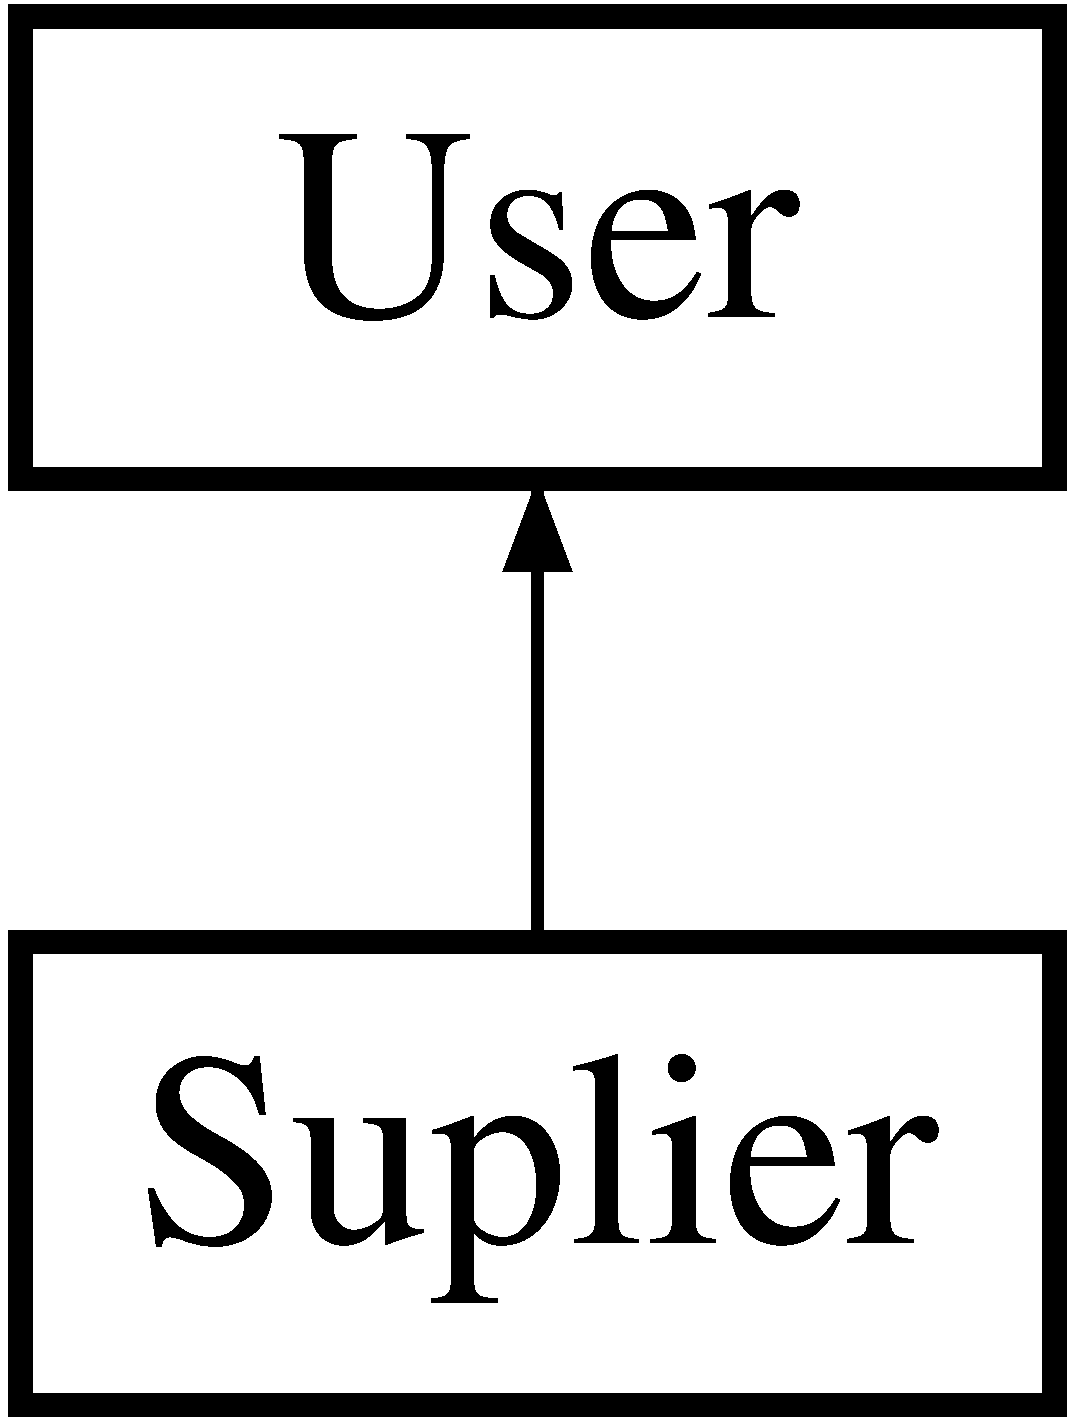
\includegraphics[height=2.000000cm]{class_suplier}
\end{center}
\end{figure}
\subsection*{Public Member Functions}
\begin{DoxyCompactItemize}
\item 
\hyperlink{class_suplier_a01702f1e6b57b187c8e0ecb06a9b2a4d}{Suplier} (string username, string password, string name, int nif, string adress)
\begin{DoxyCompactList}\small\item\em creates a new suplier \end{DoxyCompactList}\item 
\hypertarget{class_suplier_ac95a8bff3f58f427e69d88d8998853f3}{}\label{class_suplier_ac95a8bff3f58f427e69d88d8998853f3} 
void \hyperlink{class_suplier_ac95a8bff3f58f427e69d88d8998853f3}{add\+Accomodation} ()
\begin{DoxyCompactList}\small\item\em adds accomodation \end{DoxyCompactList}\item 
void \hyperlink{class_suplier_a817ef61f9a01bd480073448f1e382061}{add\+Accomodation\+File} (\hyperlink{class_accomodation}{Accomodation} $\ast$acc)
\begin{DoxyCompactList}\small\item\em adds accomodation from file \end{DoxyCompactList}\item 
\hypertarget{class_suplier_a0912f635fff680c5a321b45968c9cded}{}\label{class_suplier_a0912f635fff680c5a321b45968c9cded} 
void \hyperlink{class_suplier_a0912f635fff680c5a321b45968c9cded}{show\+Accomodations} () const
\begin{DoxyCompactList}\small\item\em shows accomodations \end{DoxyCompactList}\item 
vector$<$ \hyperlink{class_accomodation}{Accomodation} $\ast$ $>$ \hyperlink{class_suplier_a87e65aee86b034f1b4a112abb83ff53a}{get\+Accomodations} () const
\begin{DoxyCompactList}\small\item\em gets accomodations \end{DoxyCompactList}\item 
void \hyperlink{class_suplier_a9b99e7cbd4cb78a97cad39ffd6d0a691}{set\+Accomodations} (vector$<$ \hyperlink{class_accomodation}{Accomodation} $\ast$$>$ accomodations)
\begin{DoxyCompactList}\small\item\em sets accomodations \end{DoxyCompactList}\item 
string \hyperlink{class_suplier_ad6e654f4f26f6268b50f51df117793fb}{get\+Adress} () const
\begin{DoxyCompactList}\small\item\em gets adress \end{DoxyCompactList}\item 
void \hyperlink{class_suplier_a35d4dcc54e96c079ac8792806eeed739}{set\+Adress} (string adress)
\begin{DoxyCompactList}\small\item\em sets adress \end{DoxyCompactList}\item 
int \hyperlink{class_suplier_ae200d0fc598080361dccfc947dd071c5}{get\+N\+IF} () const
\begin{DoxyCompactList}\small\item\em gets N\+IF \end{DoxyCompactList}\item 
void \hyperlink{class_suplier_a91fbf47980aa9c9f3e55d9fcc0320201}{save} (ofstream \&out) const
\begin{DoxyCompactList}\small\item\em saves suplier in the file \end{DoxyCompactList}\item 
void \hyperlink{class_suplier_a2449d37d77317ea100c3d2866f8c8556}{add\+Reservation} (\hyperlink{class_reservation}{Reservation} res)
\begin{DoxyCompactList}\small\item\em adds reservation to the vector of reservations \end{DoxyCompactList}\item 
\hypertarget{class_suplier_ac455dce8b1768090654c0e5a5e840fb1}{}\label{class_suplier_ac455dce8b1768090654c0e5a5e840fb1} 
void \hyperlink{class_suplier_ac455dce8b1768090654c0e5a5e840fb1}{show\+Fees} () const
\begin{DoxyCompactList}\small\item\em displays teh percentage of the fee for each accomodation and the fees to pay for the reservations confirmed \end{DoxyCompactList}\end{DoxyCompactItemize}


\subsection{Constructor \& Destructor Documentation}
\hypertarget{class_suplier_a01702f1e6b57b187c8e0ecb06a9b2a4d}{}\label{class_suplier_a01702f1e6b57b187c8e0ecb06a9b2a4d} 
\index{Suplier@{Suplier}!Suplier@{Suplier}}
\index{Suplier@{Suplier}!Suplier@{Suplier}}
\subsubsection{\texorpdfstring{Suplier()}{Suplier()}}
{\footnotesize\ttfamily Suplier\+::\+Suplier (\begin{DoxyParamCaption}\item[{string}]{username,  }\item[{string}]{password,  }\item[{string}]{name,  }\item[{int}]{nif,  }\item[{string}]{adress }\end{DoxyParamCaption})}



creates a new suplier 


\begin{DoxyParams}{Parameters}
{\em user} & \\
\hline
{\em password} & \\
\hline
{\em name} & \\
\hline
{\em nif} & \\
\hline
\end{DoxyParams}


\subsection{Member Function Documentation}
\hypertarget{class_suplier_a817ef61f9a01bd480073448f1e382061}{}\label{class_suplier_a817ef61f9a01bd480073448f1e382061} 
\index{Suplier@{Suplier}!add\+Accomodation\+File@{add\+Accomodation\+File}}
\index{add\+Accomodation\+File@{add\+Accomodation\+File}!Suplier@{Suplier}}
\subsubsection{\texorpdfstring{add\+Accomodation\+File()}{addAccomodationFile()}}
{\footnotesize\ttfamily void Suplier\+::add\+Accomodation\+File (\begin{DoxyParamCaption}\item[{\hyperlink{class_accomodation}{Accomodation} $\ast$}]{acc }\end{DoxyParamCaption})}



adds accomodation from file 


\begin{DoxyParams}{Parameters}
{\em acc} & \\
\hline
\end{DoxyParams}
\hypertarget{class_suplier_a2449d37d77317ea100c3d2866f8c8556}{}\label{class_suplier_a2449d37d77317ea100c3d2866f8c8556} 
\index{Suplier@{Suplier}!add\+Reservation@{add\+Reservation}}
\index{add\+Reservation@{add\+Reservation}!Suplier@{Suplier}}
\subsubsection{\texorpdfstring{add\+Reservation()}{addReservation()}}
{\footnotesize\ttfamily void Suplier\+::add\+Reservation (\begin{DoxyParamCaption}\item[{\hyperlink{class_reservation}{Reservation}}]{res }\end{DoxyParamCaption})}



adds reservation to the vector of reservations 


\begin{DoxyParams}{Parameters}
{\em reservation} & \\
\hline
\end{DoxyParams}
\hypertarget{class_suplier_a87e65aee86b034f1b4a112abb83ff53a}{}\label{class_suplier_a87e65aee86b034f1b4a112abb83ff53a} 
\index{Suplier@{Suplier}!get\+Accomodations@{get\+Accomodations}}
\index{get\+Accomodations@{get\+Accomodations}!Suplier@{Suplier}}
\subsubsection{\texorpdfstring{get\+Accomodations()}{getAccomodations()}}
{\footnotesize\ttfamily vector$<$\hyperlink{class_accomodation}{Accomodation}$\ast$$>$ Suplier\+::get\+Accomodations (\begin{DoxyParamCaption}{ }\end{DoxyParamCaption}) const\hspace{0.3cm}{\ttfamily [inline]}}



gets accomodations 

\begin{DoxyReturn}{Returns}
accomodations 
\end{DoxyReturn}
\hypertarget{class_suplier_ad6e654f4f26f6268b50f51df117793fb}{}\label{class_suplier_ad6e654f4f26f6268b50f51df117793fb} 
\index{Suplier@{Suplier}!get\+Adress@{get\+Adress}}
\index{get\+Adress@{get\+Adress}!Suplier@{Suplier}}
\subsubsection{\texorpdfstring{get\+Adress()}{getAdress()}}
{\footnotesize\ttfamily string Suplier\+::get\+Adress (\begin{DoxyParamCaption}{ }\end{DoxyParamCaption}) const\hspace{0.3cm}{\ttfamily [inline]}}



gets adress 

\begin{DoxyReturn}{Returns}
adress 
\end{DoxyReturn}
\hypertarget{class_suplier_ae200d0fc598080361dccfc947dd071c5}{}\label{class_suplier_ae200d0fc598080361dccfc947dd071c5} 
\index{Suplier@{Suplier}!get\+N\+IF@{get\+N\+IF}}
\index{get\+N\+IF@{get\+N\+IF}!Suplier@{Suplier}}
\subsubsection{\texorpdfstring{get\+N\+I\+F()}{getNIF()}}
{\footnotesize\ttfamily int Suplier\+::get\+N\+IF (\begin{DoxyParamCaption}{ }\end{DoxyParamCaption}) const\hspace{0.3cm}{\ttfamily [inline]}}



gets N\+IF 

\begin{DoxyReturn}{Returns}
N\+IF 
\end{DoxyReturn}
\hypertarget{class_suplier_a91fbf47980aa9c9f3e55d9fcc0320201}{}\label{class_suplier_a91fbf47980aa9c9f3e55d9fcc0320201} 
\index{Suplier@{Suplier}!save@{save}}
\index{save@{save}!Suplier@{Suplier}}
\subsubsection{\texorpdfstring{save()}{save()}}
{\footnotesize\ttfamily void Suplier\+::save (\begin{DoxyParamCaption}\item[{ofstream \&}]{out }\end{DoxyParamCaption}) const}



saves suplier in the file 


\begin{DoxyParams}{Parameters}
{\em out} & supliers file \\
\hline
\end{DoxyParams}
\hypertarget{class_suplier_a9b99e7cbd4cb78a97cad39ffd6d0a691}{}\label{class_suplier_a9b99e7cbd4cb78a97cad39ffd6d0a691} 
\index{Suplier@{Suplier}!set\+Accomodations@{set\+Accomodations}}
\index{set\+Accomodations@{set\+Accomodations}!Suplier@{Suplier}}
\subsubsection{\texorpdfstring{set\+Accomodations()}{setAccomodations()}}
{\footnotesize\ttfamily void Suplier\+::set\+Accomodations (\begin{DoxyParamCaption}\item[{vector$<$ \hyperlink{class_accomodation}{Accomodation} $\ast$$>$}]{accomodations }\end{DoxyParamCaption})\hspace{0.3cm}{\ttfamily [inline]}}



sets accomodations 


\begin{DoxyParams}{Parameters}
{\em accomodations} & \\
\hline
\end{DoxyParams}
\hypertarget{class_suplier_a35d4dcc54e96c079ac8792806eeed739}{}\label{class_suplier_a35d4dcc54e96c079ac8792806eeed739} 
\index{Suplier@{Suplier}!set\+Adress@{set\+Adress}}
\index{set\+Adress@{set\+Adress}!Suplier@{Suplier}}
\subsubsection{\texorpdfstring{set\+Adress()}{setAdress()}}
{\footnotesize\ttfamily void Suplier\+::set\+Adress (\begin{DoxyParamCaption}\item[{string}]{adress }\end{DoxyParamCaption})\hspace{0.3cm}{\ttfamily [inline]}}



sets adress 


\begin{DoxyParams}{Parameters}
{\em adress} & \\
\hline
\end{DoxyParams}


The documentation for this class was generated from the following files\+:\begin{DoxyCompactItemize}
\item 
User.\+h\item 
User.\+cpp\end{DoxyCompactItemize}

\hypertarget{class_user}{}\section{User Class Reference}
\label{class_user}\index{User@{User}}
Inheritance diagram for User\+:\begin{figure}[H]
\begin{center}
\leavevmode
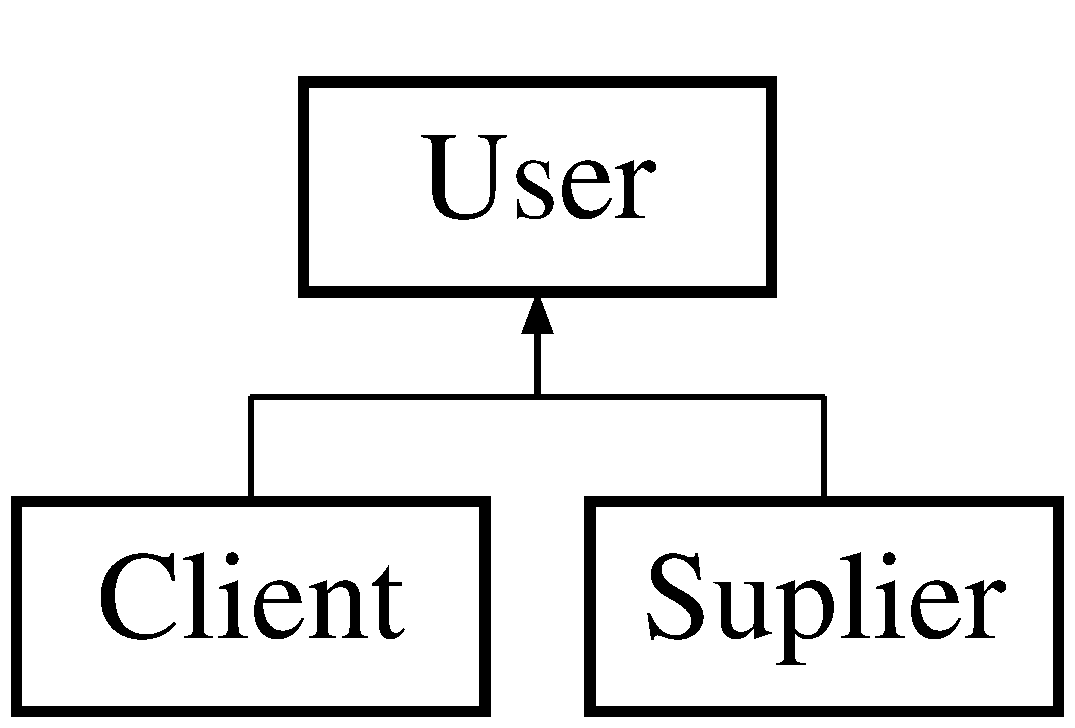
\includegraphics[height=2.000000cm]{class_user}
\end{center}
\end{figure}
\subsection*{Public Member Functions}
\begin{DoxyCompactItemize}
\item 
\hyperlink{class_user_a97b74e31502b096fb30701b8eca44f15}{User} (string username, string password, string name)
\begin{DoxyCompactList}\small\item\em \hyperlink{class_user}{User} constructor. \end{DoxyCompactList}\item 
string \hyperlink{class_user_ab9b2b5feb6bdd1582696eb6d44cee384}{get\+Name} () const
\item 
void \hyperlink{class_user_acabf7e5a40909656de5bc631abe5588c}{set\+Name} (string name)
\begin{DoxyCompactList}\small\item\em changes the name of the user \end{DoxyCompactList}\item 
string \hyperlink{class_user_a33429bdd1253091697a9c5c5e1448bee}{get\+Password} () const
\item 
void \hyperlink{class_user_ab9645a2f4dc87343f9e9aeb408be41ad}{set\+Password} (string password)
\begin{DoxyCompactList}\small\item\em changes user password \end{DoxyCompactList}\item 
string \hyperlink{class_user_a82e034043e04b2d750c654c8b2f2ce78}{get\+Username} () const
\item 
void \hyperlink{class_user_a0fed77d10cd142ee4112d650ec564e6b}{set\+Username} (string username)
\begin{DoxyCompactList}\small\item\em changes username \end{DoxyCompactList}\item 
\hypertarget{class_user_a617552867a7590074ffe76afd9dd8740}{}\label{class_user_a617552867a7590074ffe76afd9dd8740} 
void \hyperlink{class_user_a617552867a7590074ffe76afd9dd8740}{show\+Reservations} () const
\begin{DoxyCompactList}\small\item\em shows reservations \end{DoxyCompactList}\item 
vector$<$ \hyperlink{class_reservation}{Reservation} $>$ \hyperlink{class_user_ab7b3c2424a2828feb264967c3c13d2cb}{get\+Reservations} () const
\item 
\hypertarget{class_user_a042d2deaef710af2fba05abd52367e48}{}\label{class_user_a042d2deaef710af2fba05abd52367e48} 
void \hyperlink{class_user_a042d2deaef710af2fba05abd52367e48}{set\+Reservations} (vector$<$ \hyperlink{class_reservation}{Reservation} $>$ res)
\begin{DoxyCompactList}\small\item\em shows reservations \end{DoxyCompactList}\item 
void \hyperlink{class_user_a8f0bf6f9f7b1ded862b4531404068ade}{delete\+Reservation} (int position)
\begin{DoxyCompactList}\small\item\em deletes reservations \end{DoxyCompactList}\item 
bool \hyperlink{class_user_a0881b78e5e9e5040c1f5ecc0e16746b8}{operator==} (const \hyperlink{class_user}{User} \&usr) const
\begin{DoxyCompactList}\small\item\em equal operator \end{DoxyCompactList}\end{DoxyCompactItemize}


\subsection{Constructor \& Destructor Documentation}
\hypertarget{class_user_a97b74e31502b096fb30701b8eca44f15}{}\label{class_user_a97b74e31502b096fb30701b8eca44f15} 
\index{User@{User}!User@{User}}
\index{User@{User}!User@{User}}
\subsubsection{\texorpdfstring{User()}{User()}}
{\footnotesize\ttfamily User\+::\+User (\begin{DoxyParamCaption}\item[{string}]{username,  }\item[{string}]{password,  }\item[{string}]{name }\end{DoxyParamCaption})}



\hyperlink{class_user}{User} constructor. 


\begin{DoxyParams}{Parameters}
{\em username} & \\
\hline
{\em password} & \\
\hline
{\em name} & \\
\hline
\end{DoxyParams}


\subsection{Member Function Documentation}
\hypertarget{class_user_a8f0bf6f9f7b1ded862b4531404068ade}{}\label{class_user_a8f0bf6f9f7b1ded862b4531404068ade} 
\index{User@{User}!delete\+Reservation@{delete\+Reservation}}
\index{delete\+Reservation@{delete\+Reservation}!User@{User}}
\subsubsection{\texorpdfstring{delete\+Reservation()}{deleteReservation()}}
{\footnotesize\ttfamily void User\+::delete\+Reservation (\begin{DoxyParamCaption}\item[{int}]{position }\end{DoxyParamCaption})}



deletes reservations 


\begin{DoxyParams}{Parameters}
{\em position} & \\
\hline
\end{DoxyParams}
\hypertarget{class_user_ab9b2b5feb6bdd1582696eb6d44cee384}{}\label{class_user_ab9b2b5feb6bdd1582696eb6d44cee384} 
\index{User@{User}!get\+Name@{get\+Name}}
\index{get\+Name@{get\+Name}!User@{User}}
\subsubsection{\texorpdfstring{get\+Name()}{getName()}}
{\footnotesize\ttfamily string User\+::get\+Name (\begin{DoxyParamCaption}{ }\end{DoxyParamCaption}) const\hspace{0.3cm}{\ttfamily [inline]}}

\begin{DoxyReturn}{Returns}
name of the user 
\end{DoxyReturn}
\hypertarget{class_user_a33429bdd1253091697a9c5c5e1448bee}{}\label{class_user_a33429bdd1253091697a9c5c5e1448bee} 
\index{User@{User}!get\+Password@{get\+Password}}
\index{get\+Password@{get\+Password}!User@{User}}
\subsubsection{\texorpdfstring{get\+Password()}{getPassword()}}
{\footnotesize\ttfamily string User\+::get\+Password (\begin{DoxyParamCaption}{ }\end{DoxyParamCaption}) const\hspace{0.3cm}{\ttfamily [inline]}}

\begin{DoxyReturn}{Returns}
password of the user 
\end{DoxyReturn}
\hypertarget{class_user_ab7b3c2424a2828feb264967c3c13d2cb}{}\label{class_user_ab7b3c2424a2828feb264967c3c13d2cb} 
\index{User@{User}!get\+Reservations@{get\+Reservations}}
\index{get\+Reservations@{get\+Reservations}!User@{User}}
\subsubsection{\texorpdfstring{get\+Reservations()}{getReservations()}}
{\footnotesize\ttfamily vector$<$\hyperlink{class_reservation}{Reservation}$>$ User\+::get\+Reservations (\begin{DoxyParamCaption}{ }\end{DoxyParamCaption}) const\hspace{0.3cm}{\ttfamily [inline]}}

\begin{DoxyReturn}{Returns}
reservations 
\end{DoxyReturn}
\hypertarget{class_user_a82e034043e04b2d750c654c8b2f2ce78}{}\label{class_user_a82e034043e04b2d750c654c8b2f2ce78} 
\index{User@{User}!get\+Username@{get\+Username}}
\index{get\+Username@{get\+Username}!User@{User}}
\subsubsection{\texorpdfstring{get\+Username()}{getUsername()}}
{\footnotesize\ttfamily string User\+::get\+Username (\begin{DoxyParamCaption}{ }\end{DoxyParamCaption}) const\hspace{0.3cm}{\ttfamily [inline]}}

\begin{DoxyReturn}{Returns}
username 
\end{DoxyReturn}
\hypertarget{class_user_a0881b78e5e9e5040c1f5ecc0e16746b8}{}\label{class_user_a0881b78e5e9e5040c1f5ecc0e16746b8} 
\index{User@{User}!operator==@{operator==}}
\index{operator==@{operator==}!User@{User}}
\subsubsection{\texorpdfstring{operator==()}{operator==()}}
{\footnotesize\ttfamily bool User\+::operator== (\begin{DoxyParamCaption}\item[{const \hyperlink{class_user}{User} \&}]{usr }\end{DoxyParamCaption}) const}



equal operator 


\begin{DoxyParams}{Parameters}
{\em user} & \\
\hline
\end{DoxyParams}
\begin{DoxyReturn}{Returns}
if it went well 
\end{DoxyReturn}
\hypertarget{class_user_acabf7e5a40909656de5bc631abe5588c}{}\label{class_user_acabf7e5a40909656de5bc631abe5588c} 
\index{User@{User}!set\+Name@{set\+Name}}
\index{set\+Name@{set\+Name}!User@{User}}
\subsubsection{\texorpdfstring{set\+Name()}{setName()}}
{\footnotesize\ttfamily void User\+::set\+Name (\begin{DoxyParamCaption}\item[{string}]{name }\end{DoxyParamCaption})\hspace{0.3cm}{\ttfamily [inline]}}



changes the name of the user 


\begin{DoxyParams}{Parameters}
{\em name} & \\
\hline
\end{DoxyParams}
\hypertarget{class_user_ab9645a2f4dc87343f9e9aeb408be41ad}{}\label{class_user_ab9645a2f4dc87343f9e9aeb408be41ad} 
\index{User@{User}!set\+Password@{set\+Password}}
\index{set\+Password@{set\+Password}!User@{User}}
\subsubsection{\texorpdfstring{set\+Password()}{setPassword()}}
{\footnotesize\ttfamily void User\+::set\+Password (\begin{DoxyParamCaption}\item[{string}]{password }\end{DoxyParamCaption})\hspace{0.3cm}{\ttfamily [inline]}}



changes user password 


\begin{DoxyParams}{Parameters}
{\em password} & \\
\hline
\end{DoxyParams}
\hypertarget{class_user_a0fed77d10cd142ee4112d650ec564e6b}{}\label{class_user_a0fed77d10cd142ee4112d650ec564e6b} 
\index{User@{User}!set\+Username@{set\+Username}}
\index{set\+Username@{set\+Username}!User@{User}}
\subsubsection{\texorpdfstring{set\+Username()}{setUsername()}}
{\footnotesize\ttfamily void User\+::set\+Username (\begin{DoxyParamCaption}\item[{string}]{username }\end{DoxyParamCaption})\hspace{0.3cm}{\ttfamily [inline]}}



changes username 


\begin{DoxyParams}{Parameters}
{\em username} & \\
\hline
\end{DoxyParams}


The documentation for this class was generated from the following files\+:\begin{DoxyCompactItemize}
\item 
User.\+h\item 
User.\+cpp\end{DoxyCompactItemize}

\hypertarget{class_wrong_option}{}\section{Wrong\+Option Class Reference}
\label{class_wrong_option}\index{Wrong\+Option@{Wrong\+Option}}
\subsection*{Public Member Functions}
\begin{DoxyCompactItemize}
\item 
\hypertarget{class_wrong_option_ad167d8d4a022b1069a78b0be521cb09f}{}\label{class_wrong_option_ad167d8d4a022b1069a78b0be521cb09f} 
{\bfseries Wrong\+Option} (uns\+Int min, uns\+Int max)
\end{DoxyCompactItemize}
\subsection*{Friends}
\begin{DoxyCompactItemize}
\item 
\hypertarget{class_wrong_option_a272717a9c47de3cdf605f30ccc0b7c08}{}\label{class_wrong_option_a272717a9c47de3cdf605f30ccc0b7c08} 
ostream \& {\bfseries operator$<$$<$} (ostream \&out, \hyperlink{class_wrong_option}{Wrong\+Option} \&wo)
\end{DoxyCompactItemize}


The documentation for this class was generated from the following file\+:\begin{DoxyCompactItemize}
\item 
utils.\+h\end{DoxyCompactItemize}

%--- End generated contents ---

% Index
\backmatter
\newpage
\phantomsection
\clearemptydoublepage
\addcontentsline{toc}{chapter}{Index}
\printindex

\end{document}
